\documentclass{article}

\usepackage{polski}
\usepackage[utf8]{inputenc}

\usepackage[margin=0.75in]{geometry}

\usepackage{graphicx} % Required for inserting images
\usepackage{amsmath}
\usepackage{amssymb}
\usepackage{float}

\title{
    Teoria Sterowania\\
    \Large Portrety Fazowe
}
\author{Maciej Różewicz}
\date{2025}

\makeatletter         
\def\@maketitle{
\raggedright
\begin{center}
    \includegraphics[width=0.5\linewidth]{fig/agh_logo.PNG}\\[8ex]
\end{center}
\begin{center}
    {\huge \bfseries \sffamily \@title }\\[4ex] 
    {\large  \@author}\\[4ex] 
    \@date\\[8ex]
\end{center}}
\makeatother

\begin{document}
\maketitle

%%%%%%%%%%%%%%%%%%%%%%%%%%%%%%%%%%%%%%%%%%%%%%%%%%%%%%%%%%%%
\newpage
\section{Cel ćwiczenia}
Celem ćwiczenia jest zapoznanie się z metodą analizy układów dynamicznych wykorzystującą jej tzw. portret fazowy.
W czasie ćwiczeń analizowane będą układy liniowe drugiego rzędu.

W czasie ćwiczenia należy zwrócić uwagę na wpływ pierwiastków wielomianu charakterystycznego i jego współczynników na kształt powstających portretów fazowych.

\section{Portrety fazowe - wprowadzenie}
Metoda portretów fazowych (płaszczyzny fazowej) polega na badaniu trajektorii autonomicznego układu dynamicznego
\begin{equation} \label{eq:system_nonlin}
    \dot{X}(t) = f(X(t))
\end{equation}
w układzie współrzędnych $(x, \dot{x}, \cdots x^{(n-1)})$.
Jest to metoda dokładna, dająca pełną informację o przebiegach czasowych układu, dla układów do drugiego rzędu włącznie.
Można ją stosować dla układów o rzędzie wyższym, lecz ze względów praktycznych wymaga to aproksymacji układem rzędu drugiego.
Inaczej już w przypadku układu rzędu 3. występują bardzo duże trudności w~analizie wyników.

\textbf{Przestrzenią fazową} $n$-wymiarową nazywamy przestrzeń, kórej elementami są wektory o składowych będących kolejnymi pochodnymi wzglem czasu pierwszej składowej:
$$
    \begin{bmatrix}
        x   &   x^{(1)} &   \cdots  &   x^{(n-1)}
    \end{bmatrix}^{T}
$$
gdzie:
\begin{itemize}
    \item $n$ - rząd układu,
    \item $x$ - wielkość charakterystyczna dla danego układu - najczęściej wartość regulowana lub uchyb sterowania.
\end{itemize}

\textbf{Trajektorią fazową} nazywamy rzut wykresu rozwiązania równania (\ref{eq:system_nonlin}) z~przestrzeni $\mathbb{R}^{n} \times \mathbb{R}_{+}$ na przestrzeń fazową układu. Każdemu stanowi układu odpowiada zatem jeden punkt w przestrzeni fazowej, a zmiana stanu jest odwzorowana poprzez ruch tego punktu wzdłuż krzywych, którymi są trajektorie fazowe.

\begin{figure}[H]
    \centering
    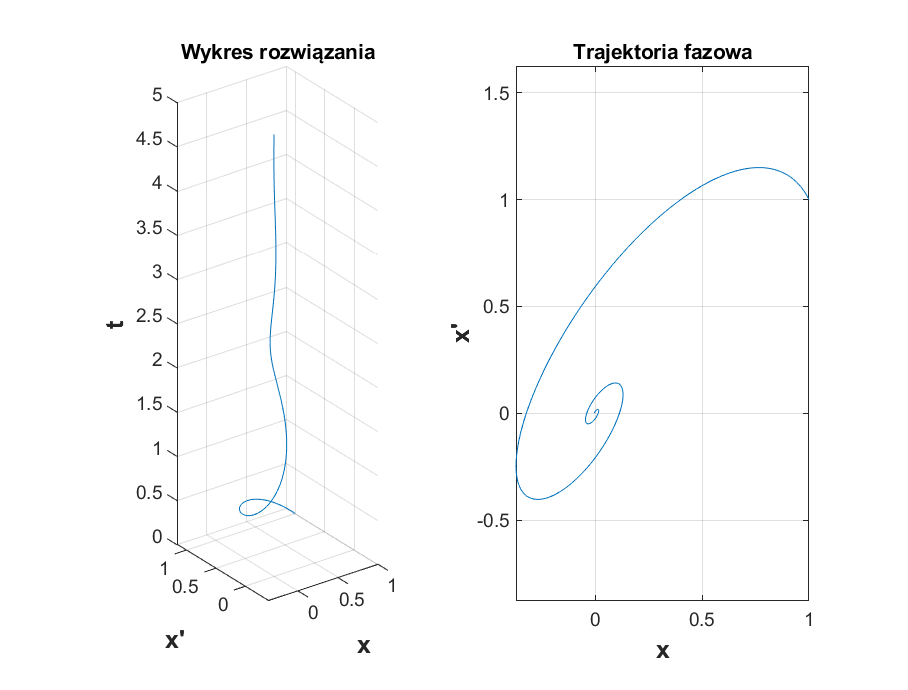
\includegraphics[width=0.7\linewidth]{fig/01_portrety_fazowe/wykres_vs_trajektoria_fazowa.eps}
    \caption{Wykres rozwiązania równania (\ref{eq:system_nonlin}) i jego trajektoria fazowa.}
    \label{fig:enter-label}
\end{figure}

\textbf{Portretem fazowym} nazywamy rodzinę trajektorii fazowych dla wszystkich możliwych warunków początkowych układu.

    %=======================================================
    \subsection{Skala czasu na portrecie fazowym}
    Rzutowanie trajektorii rozwiązania na płaszczyznę fazową powoduje utratę bezpośredniej informacji o czasie - pozostaje jedynie informacja o kierunkach zmian stanu.
    Jednak na podstawie \textbf{trajektorii fazowej} można tę informację częściowo odtworzyć.
    Wykorzystuje się do tego fakt, że każdy punkt trajektorii fazowej jest związany z jednym punktem czasowym, oraz zależność:
    $$
        \dot{x} = \frac{dx}{dt}.
    $$
    Przekształcając i całkując powyższe równanie otrzymuje się wyrażenie na czas przejścia między punktami $x_{1}$ i $x_{2}$:
    \begin{equation} \label{eq:czas}
        t = \int_{x_{1}}^{x_{2}}{\frac{dx}{\dot{x}}}.
    \end{equation}
    Znając analityczną zależność na $\dot{x}$ w funkcji $x$ można tę całkę wyznaczyć dokładnie.
    Lecz w praktyce stosuje się przybliżenie trajektorii fazowej odcinkami prostoliniowymi:
    \begin{figure}[H]
        \centering
        \includegraphics[width=0.75\linewidth]{fig/01_portrety_fazowe/czas.eps}
        \caption{Aproksymacja trajektorii fazowej odcinkami.}
        \label{fig:enter-label}
    \end{figure}
    Wówczas całkę (\ref{eq:czas}) można zastąpić zależnością przyrostową:
    \begin{equation} \label{eq:czas_d}
        \Delta t = \frac{\Delta x}{\dot{x}_{mean}}
    \end{equation}
    gdzie:
    \begin{itemize}
        \item $\Delta x = |x_{2} - x_{1}|$ - długość przedziału aproksymacji,
        \item $\dot{x}_{mean}$ - średnia wartość $\dot{x}$ w przedziale $(x_{1}, x_{2})$.
    \end{itemize}
    Dość łatwo zauważyć, że aproksymacja ta będzie dokładna, gdy trajektoria będzie równoległa do osi $x$ (ponieważ $\dot{x}_{mean}$ jest dokładną wartością $\dot{x}$), a błąd aproksymacji będzie rósł im trajektoria fazowa jest "bardziej pionowa".

    Można zadać sobie również pytanie odwrotne: gdzie układ będzie po czasie $\Delta t$?
    Można zauważyć, że wartość średnią "prędkości" można zapisać jako:
    $$
        \dot{x}_{mean} = \dot{x}(0) + \frac{\Delta \dot{x}}{2},
    $$
    zatem biorąc pod uwagę równanie (\ref{eq:czas_d}) otrzymuje się:
    $$  
        \frac{\Delta x}{\Delta t} = \frac{2\dot{x}(0) + \Delta \dot{x}}{2}
    $$
    $$
        \frac{2}{\Delta t} = \frac{2\dot{x}(0) + \Delta \dot{x}}{\Delta x}
    $$
    Z interpretacji geometrycznej na rysunku \ref{fig:czas} można zauważyć, że:
    $$
        \beta = \arctan{\frac{2}{\Delta t}}
    $$
    \begin{figure}[H]
        \centering
        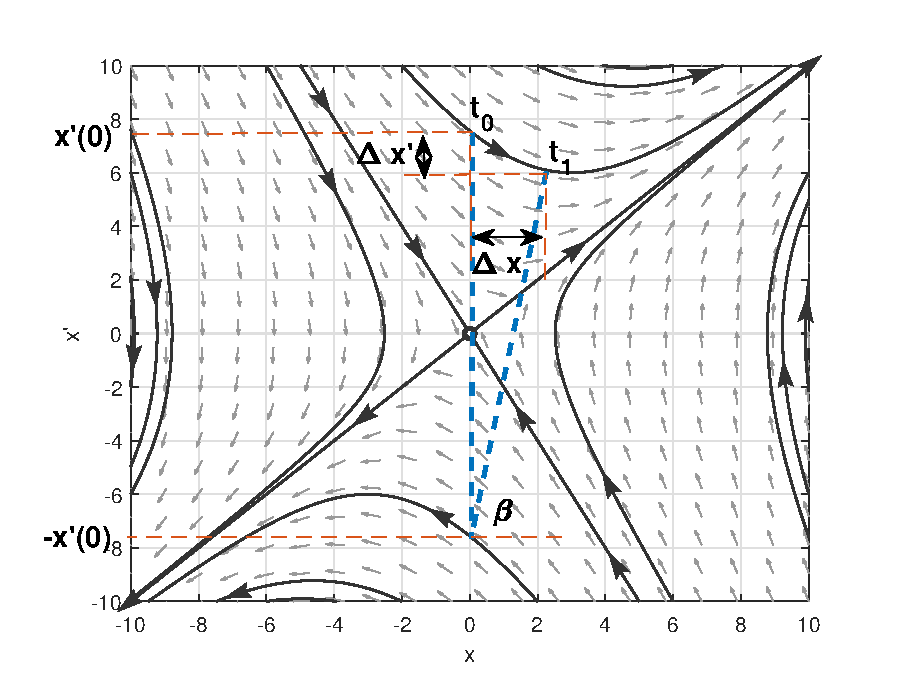
\includegraphics[width=0.75\linewidth]{fig/01_portrety_fazowe/czas_2.eps}
        \caption{Graficzna konstrukcja przyrostu trajektorii w czasie $\Delta t = t_{1} - t_{0}$.}
        \label{fig:czas}
    \end{figure}

    %=======================================================
    \subsection{Konstrukcja portretów fazowych}
    Portrety fazowe można konstruować poprzez rozwiązanie równania (\ref{eq:system_nonlin}) dla wielu punktów początkowych i wyrysowanie ich na płaszczyźnie fazowej.
    W przypadku ogólnym - równania nieliniowego, wykonywane będzie to w ogólności numerycznie.
    Natomiast dla rozważanego przypadku równania liniowego można je stosunkowo łatwo rozwiązać analitycznie - w funkcji czasu, lub jako zależność $\dot{x}(x)$.

    Istnieją jednak inne metody pozwalające konstruować przybliżone portrety fazowe, bez rozwiązywania równań różniczkowych układu.
    Są to np:
    \begin{itemize}
        \item metoda izoklin,
        \item metoda Pella,
        \item metoda delta.
    \end{itemize}
    Tutaj przedstawiona będzie tylko pierwsza z nich.

        %------------------------------------------------------
        \subsubsection{Metoda izoklin}
        Metoda izoklin polega na przekształcaniu równania układu dla uzyskania linii stałego nachylenia trajektorii fazowych.
        Przy zadanych warunkach początkowych umożliwia to wykreślenie trajektorii fazowej układu bez rozwiązywania równań układu.
        Na przykład rozważając układ:
        $$
            \ddot{x} + 2\xi\omega_{0}\dot{x} + x = 0
        $$
        Wprowadzamy współrzędne fazowe:
        $$
            x_{1} = x, \, x_{2} = \dot{x} = \frac{d x_{1}}{dt}
        $$
        Po zmianie zmiennych otrzymujemy postać:
        $$
            \frac{dx_{2}}{dt} + 2\xi\omega_{0}x_{2} + x_{1} = 0
        $$
        Dzieląc równanie przez $x_{2}$ (i pamiętając, że $x_{2} = \frac{d x_{1}}{dt}$) i przyrównując wynik do stałej otrzymuje się równanie krzywej, gdzie na której trajektoria fazowa ma stałe nachylenie:
        $$
            \frac{dx_{2}}{dx_{1}} = -\frac{x_{1} + 2\xi\omega_{0}x_{2}}{x_{2}} = C
        $$

        Zatem aby odnaleźć punkty o nachyleniu krzywej równym $C$ wyznaczamy prostą:
        $$
            x_{2} = -\frac{1}{C + 2\xi\omega_{0}}x_{2}
        $$

        \begin{figure}[H]
            \centering
            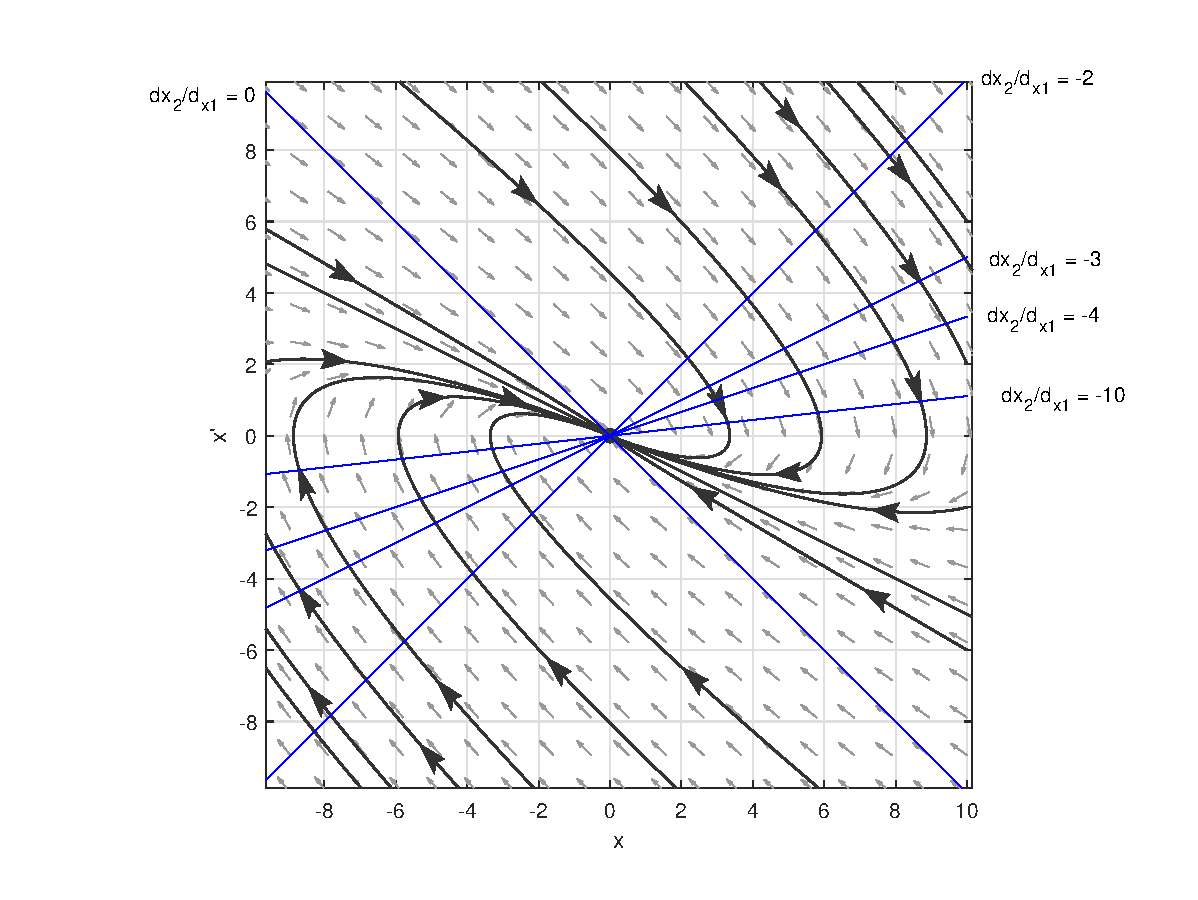
\includegraphics[width=0.75\linewidth]{fig/01_portrety_fazowe/izokliny.eps}
            \caption{Prezentacja metody izoklin.}
            \label{fig:enter-label}
        \end{figure}
        
    %=======================================================
    \subsection{Portrety fazowe układów liniowych}
    W przypadku układów liniowych równanie (\ref{eq:system_nonlin}) przyjmuje postać:
    \begin{equation} \label{eq:system_lin}
        \dot{X}(t) = AX(t)
    \end{equation}
    gdzie:
    \begin{itemize}
        \item $A \in \mathbb{R}^{n}$ - stała macierz przejścia (transformacji) systemu liniowego - w rozważanych przypadkach $n = 2$,
        \item $X(t) = \begin{bmatrix} x_{1}(t)  & x_{2}(t) \end{bmatrix}^{T}$
    \end{itemize}

    Taki układ liniowy można zapisać w postaci jednego równania drugiego stopnia:
    \begin{equation} \label{eq:eq_2nd}
        \ddot{x} + 2 \xi \omega_{0} \dot{x} + \omega_{0}^{2} x = 0
    \end{equation}
    \begin{itemize}
        \item $\xi$ - tłumienie względne,
        \item $\omega_{0}$ - częstotliwość drgań własnych,
        \item $x = x_{1}$.
    \end{itemize}
    Z odpowiadającą mu macierzą $A$:
    \begin{equation} \label{eq:a_frobenius}
        A
        =
        \begin{bmatrix}
            0               &   1\\
            -\omega_{0}^{2} &   -2\xi\omega_{0}
        \end{bmatrix}	
    \end{equation}
    Czyli w postaci Frobeniusa.

    Można zauważyć, że kształt trajektorii fazowych będzie zdeterminowany przez rozkład wartości własnych macierzy (\ref{eq:a_frobenius}):
    \begin{equation}
        \lambda_{1,2} = -\xi\omega_{0} \pm \sqrt{\xi^{2} - 1}
    \end{equation}
    W zależności od rozłożenia tych wartości własnej na płaszczyźnie zespolonej można wyznaczyć 9 typów portretów fazowych.
    
        %------------------------------------------------------
        \subsubsection{Centrum - 2 pierwiastki czysto urojone}
        Aby istniały dwa pierwiastki czysto urojone muszą zachodzić warunki:
        \begin{itemize}
            \item $\xi\omega_{0} = 0 \rightarrow \xi = 0$ - brak tłumienia,
            \item $\omega_{0}^{2} > 0$.
        \end{itemize}

        \begin{figure}[H]
            \centering
            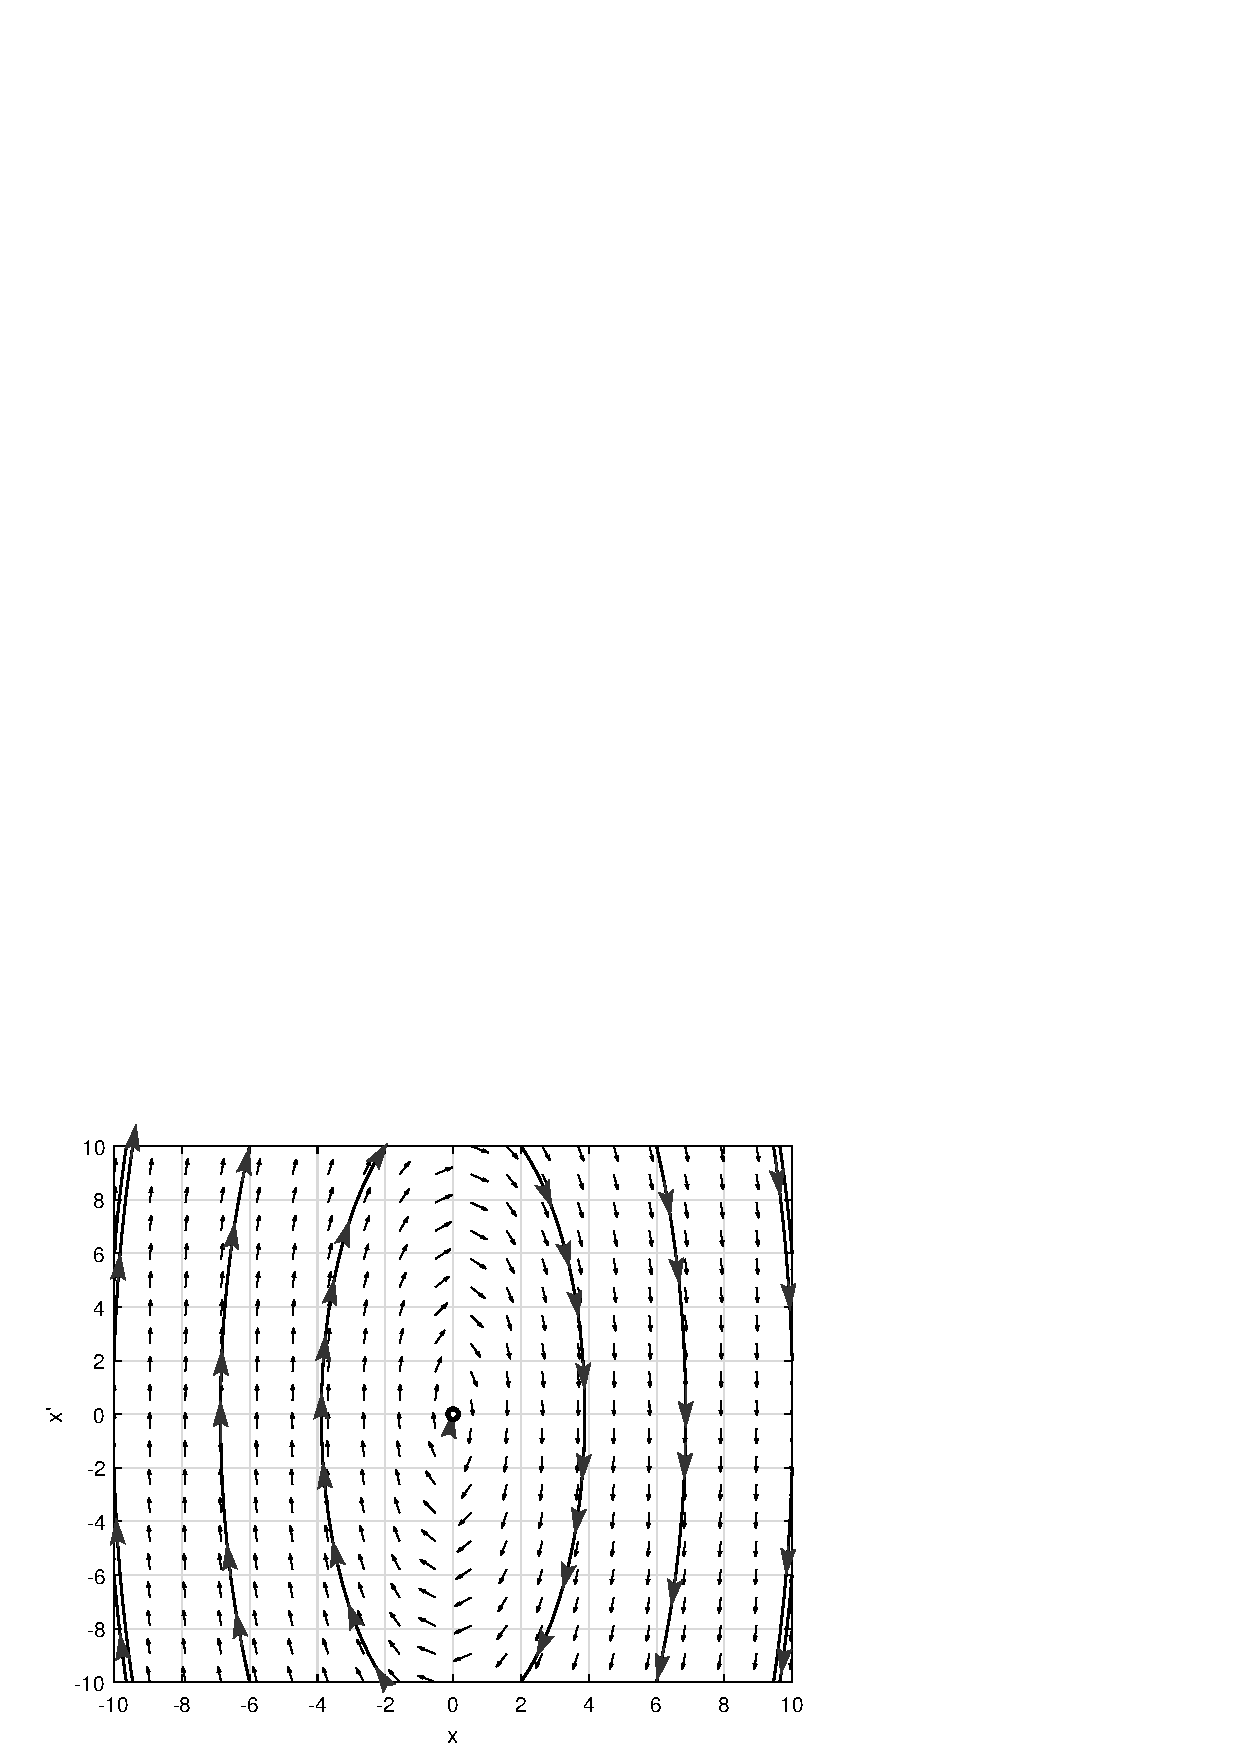
\includegraphics[width=0.5\linewidth]{fig/01_portrety_fazowe/centrum.PNG}
            \caption{Ułożenie wartości własnych dla portretu typu \textbf{centrum}.}
            \label{fig:enter-label}
        \end{figure}

        \begin{figure}[H]
            \centering
            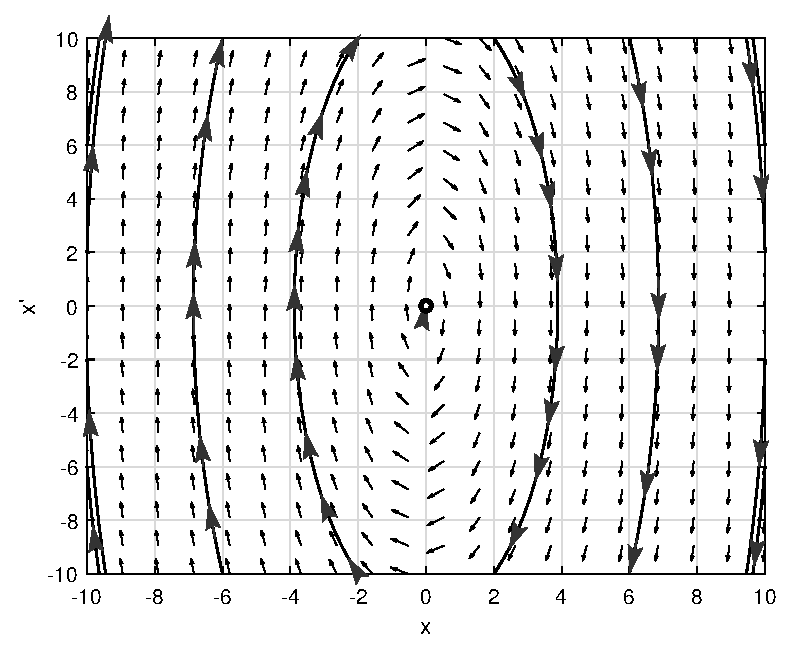
\includegraphics[width=0.75\linewidth]{fig/01_portrety_fazowe/centrum.eps}
            \caption{Przykładowy portret fazowy dla portretu typu \textbf{centrum}.}
            \label{fig:enter-label}
        \end{figure}

        \begin{figure}[H]
            \centering
            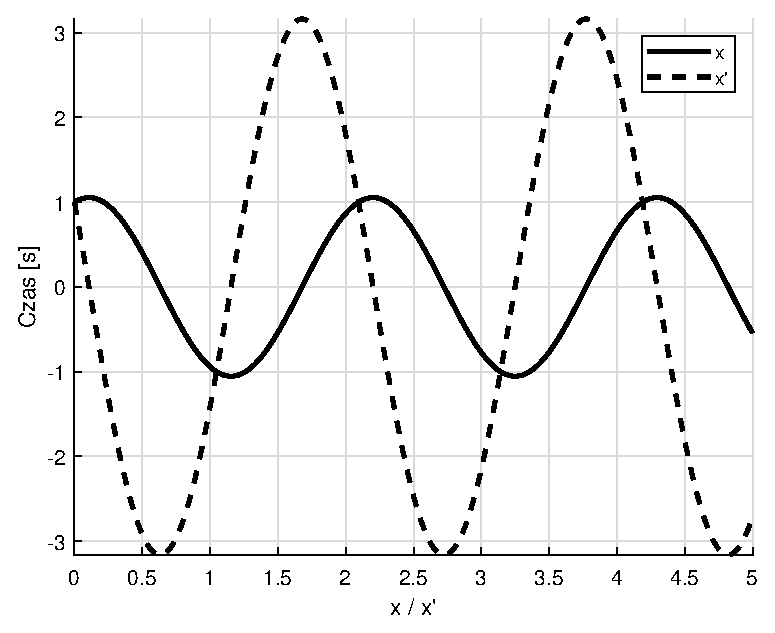
\includegraphics[width=0.5\linewidth]{fig/01_portrety_fazowe/centrum_wykres.eps}
            \caption{Przykładowe przebiegi czasowe dla portretu typu \textbf{centrum}.}
            \label{fig:enter-label}
        \end{figure}
        
        %------------------------------------------------------
        \subsubsection{Ognisko stabilne - 2 pierwiastki zespolone, stabilne}
        Aby istniały dwa pierwiastki zespolone, stabilne muszą zachodzić warunki:
        \begin{itemize}
            \item $0 < \xi < 1$ - tłumienie,
            \item $\omega_{0} > 0$.
        \end{itemize}

        \begin{figure}[H]
            \centering
            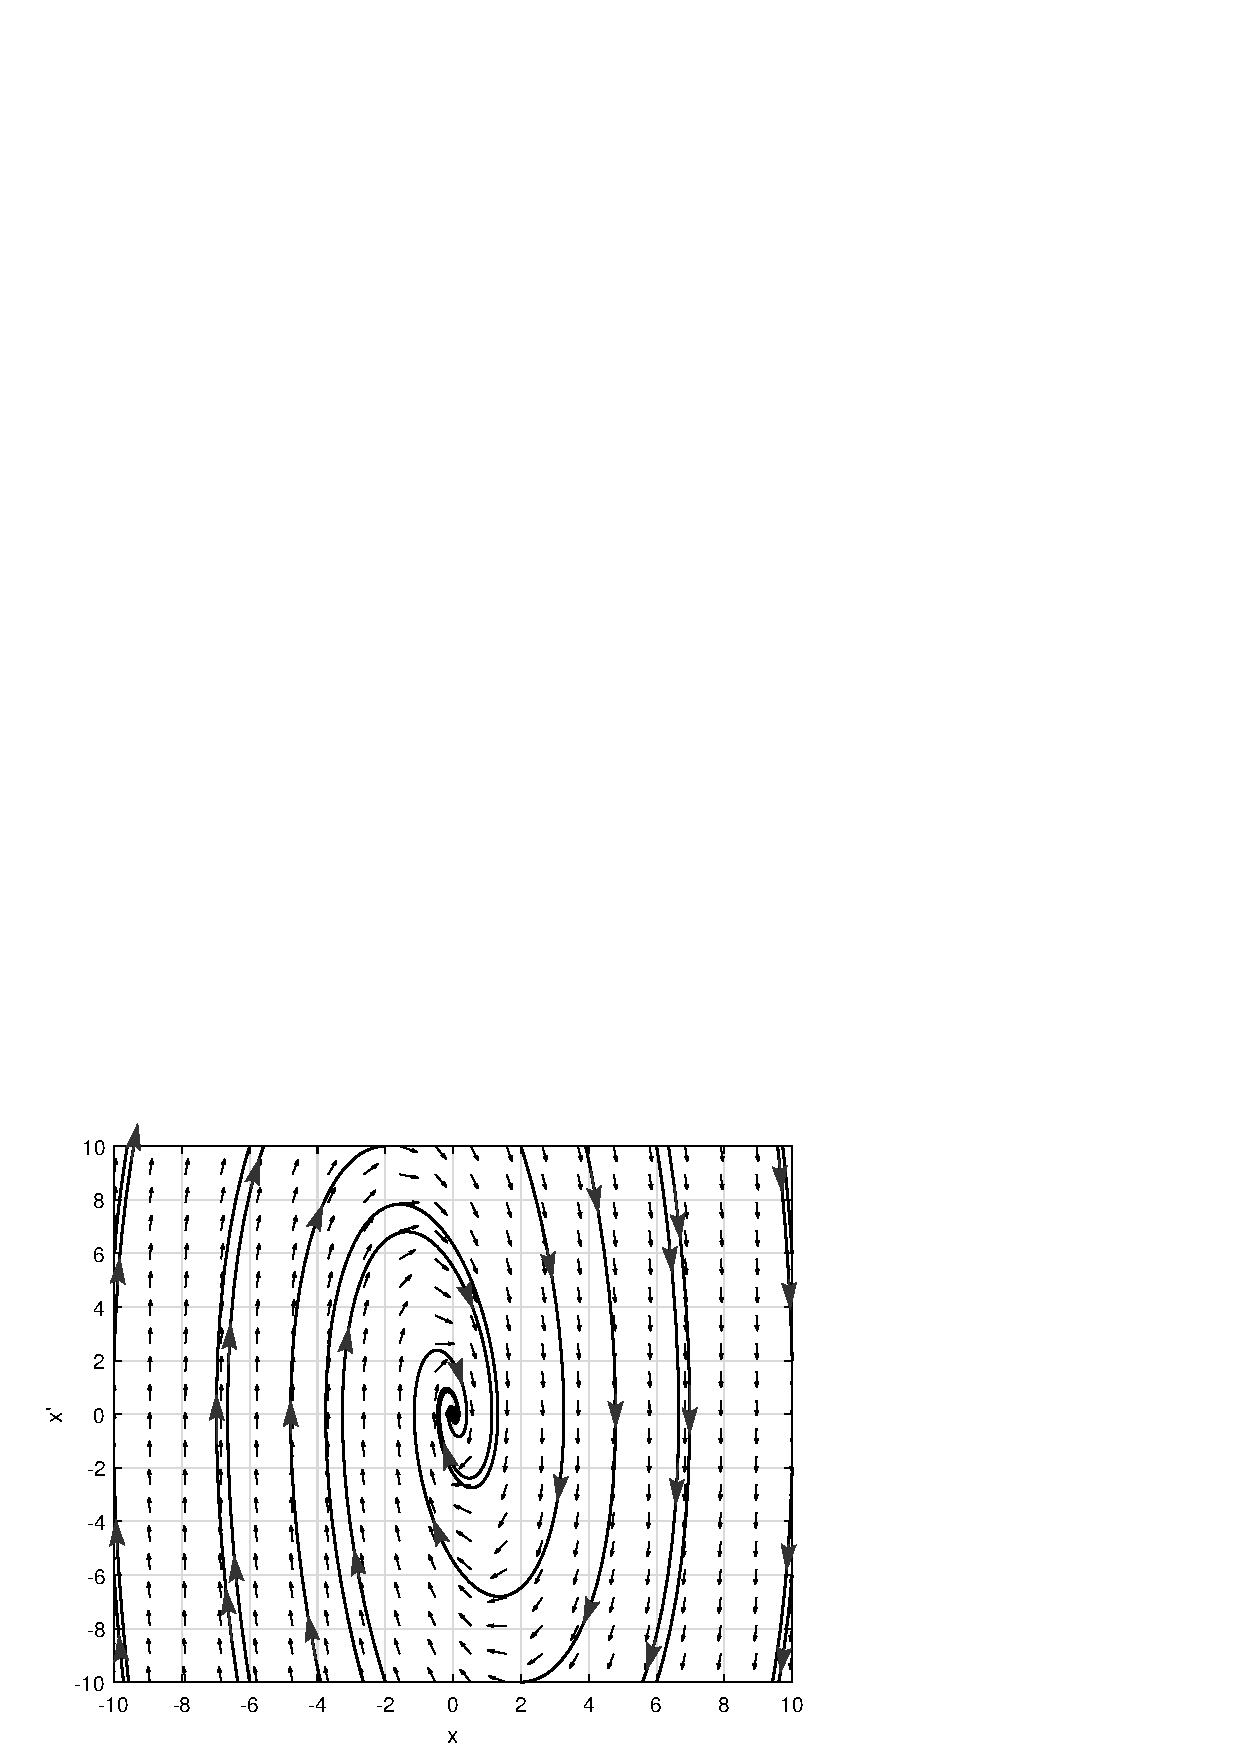
\includegraphics[width=0.5\linewidth]{fig/01_portrety_fazowe/ognisko_stabilne.PNG}
            \caption{Ułożenie wartości własnych dla portretu typu \textbf{ognisko stabilne}.}
            \label{fig:enter-label}
        \end{figure}

        \begin{figure}[H]
            \centering
            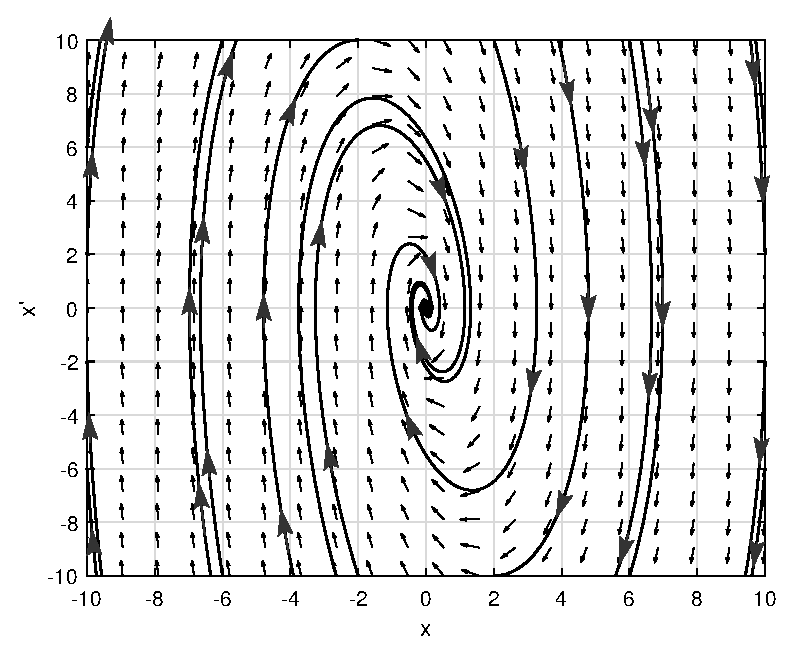
\includegraphics[width=0.75\linewidth]{fig/01_portrety_fazowe/ognisko_stabilne.eps}
            \caption{Przykładowy portret fazowy dla portretu typu \textbf{ognisko stabilne}.}
            \label{fig:enter-label}
        \end{figure}
    
        \begin{figure}[H]
            \centering
            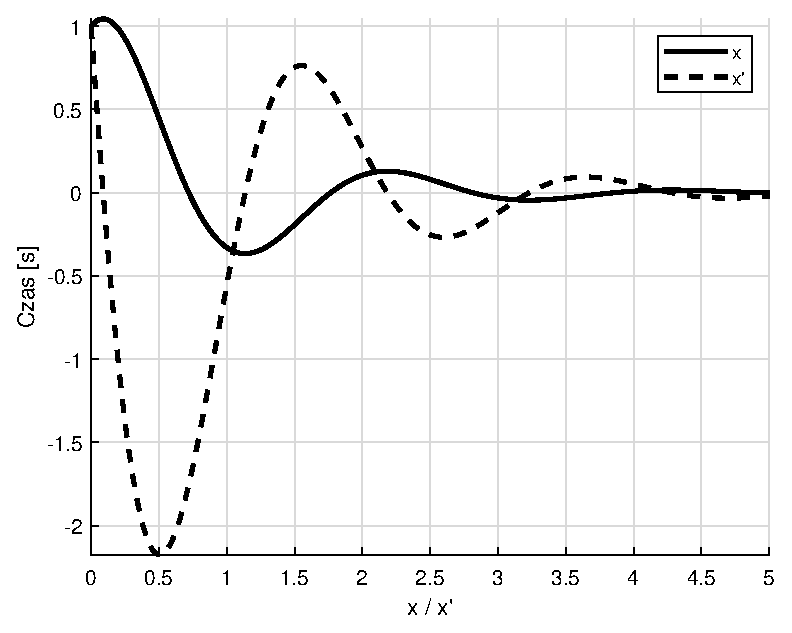
\includegraphics[width=0.5\linewidth]{fig/01_portrety_fazowe/ognisko_stabilne_wykres.eps}
            \caption{Przykładowe przebiegi czasowe dla portretu typu \textbf{ognisko stabilne}.}
            \label{fig:enter-label}
        \end{figure}

        %------------------------------------------------------
        \subsubsection{Ognisko niestabilne - 2 pierwiastki zespolone, niestabilne}
        Aby istniały dwa pierwiastki zespolone, niestabilne muszą zachodzić warunki:
        \begin{itemize}
            \item $-1 < \xi < 0$ - tłumienie,
            \item $\omega_{0} > 0$.
        \end{itemize}

        \begin{figure}[H]
            \centering
            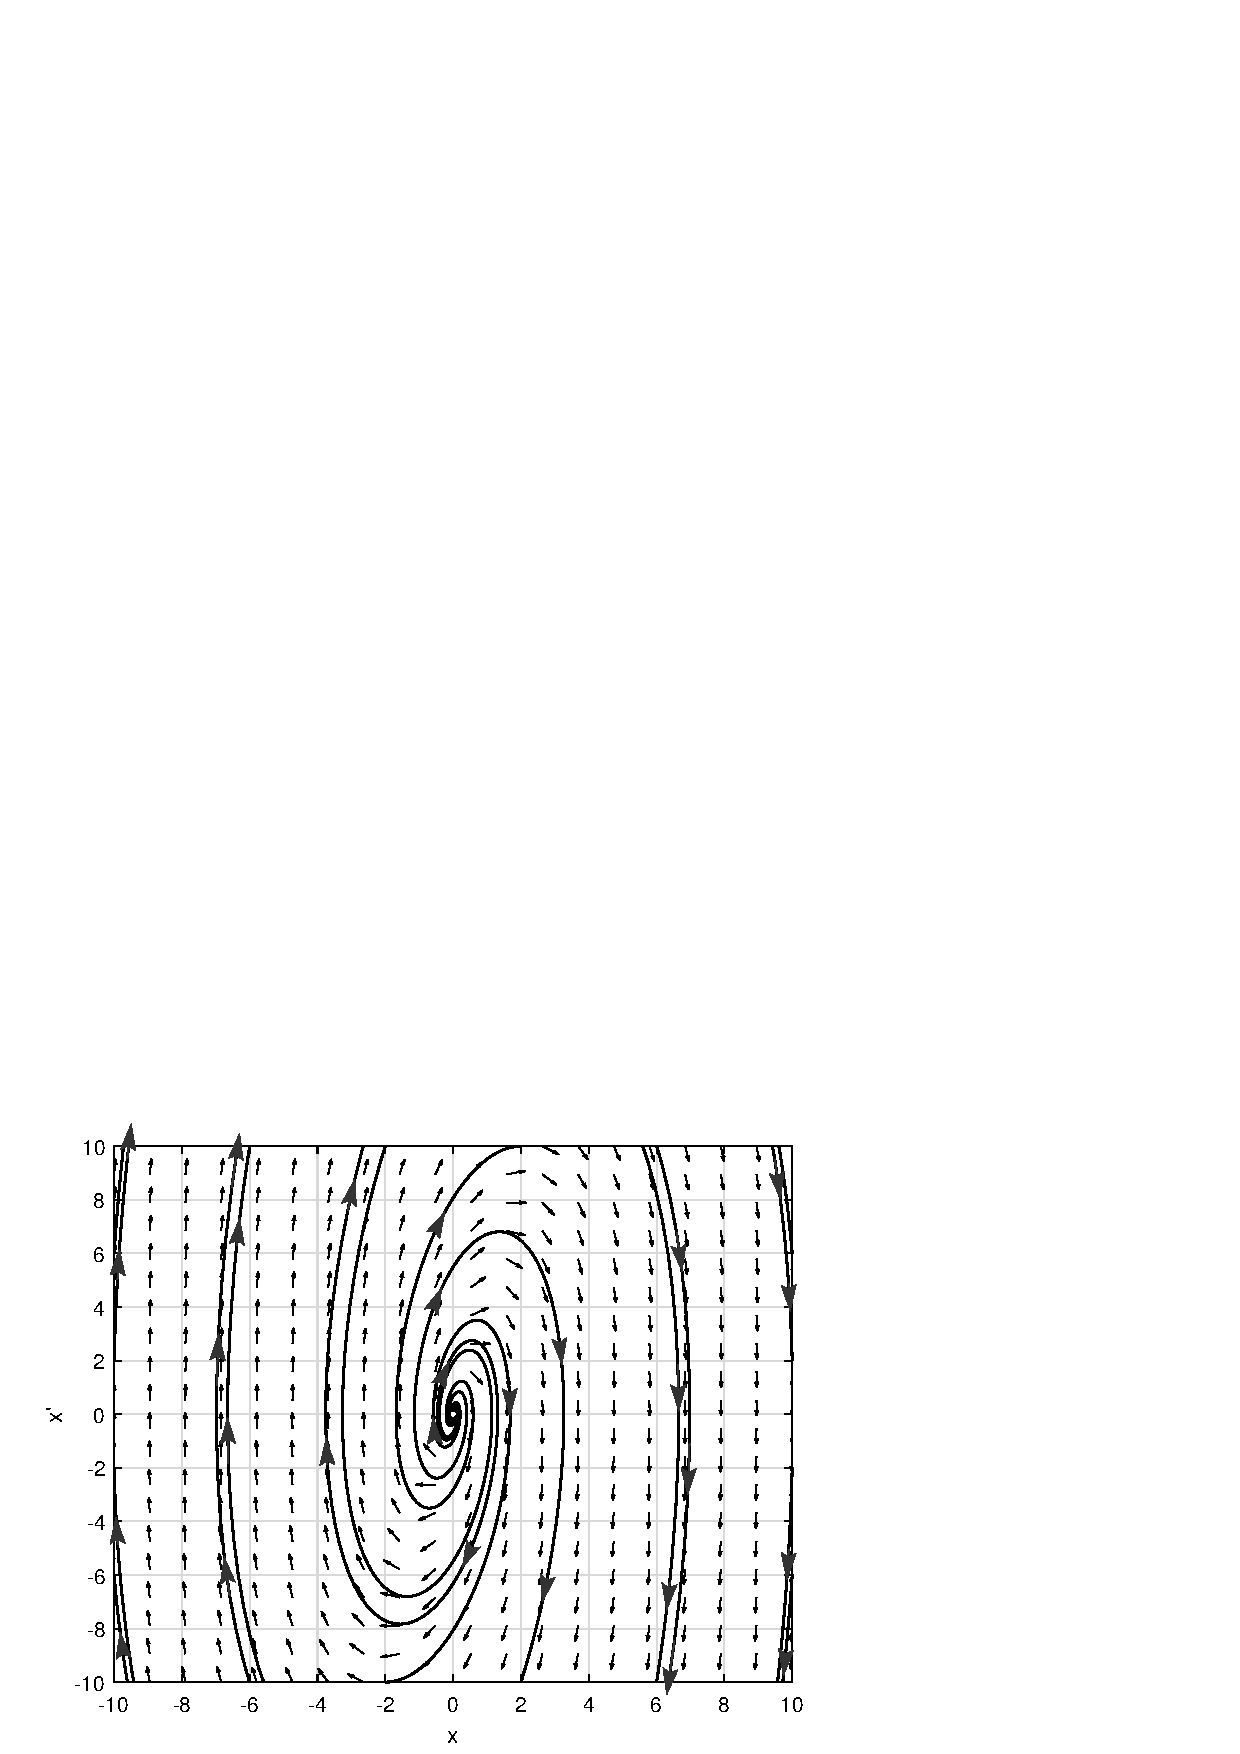
\includegraphics[width=0.5\linewidth]{fig/01_portrety_fazowe/ognisko_niestabilne.PNG}
            \caption{Ułożenie wartości własnych dla portretu typu \textbf{ignisko niestabilne}.}
            \label{fig:enter-label}
        \end{figure}

        \begin{figure}[H]
            \centering
            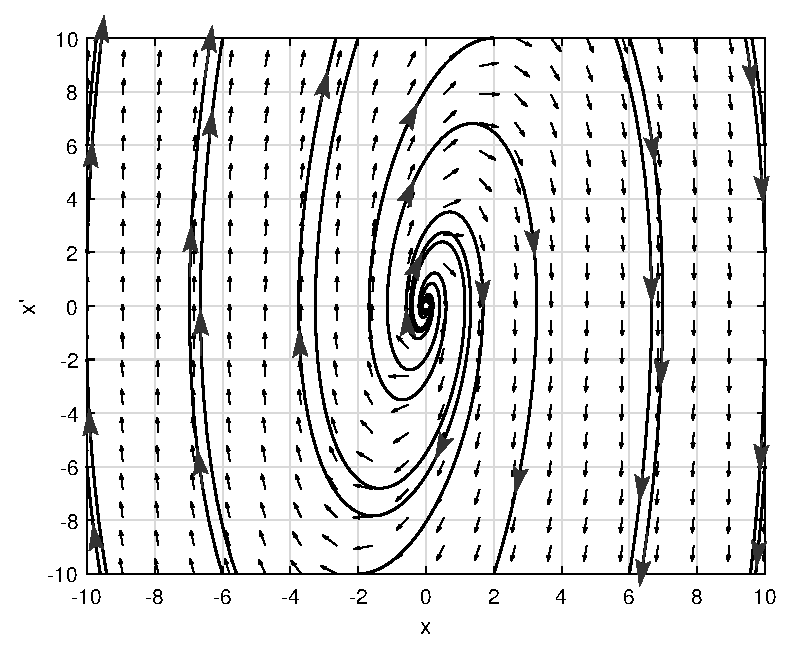
\includegraphics[width=0.75\linewidth]{fig/01_portrety_fazowe/ognisko_niestabilne.eps}
            \caption{Przykładowy portret fazowy dla portretu typu \textbf{ognisko niestabilne}.}
            \label{fig:enter-label}
        \end{figure}

        \begin{figure}[H]
            \centering
            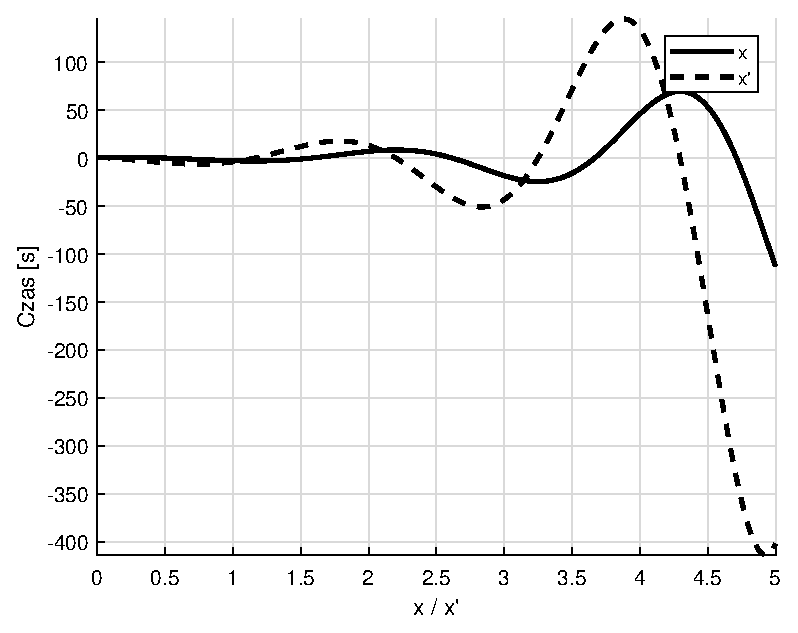
\includegraphics[width=0.5\linewidth]{fig/01_portrety_fazowe/ognisko_niestabilne_wykres.eps}
            \caption{Przykładowe przebiegi czasowe dla portretu typu \textbf{ognisko niestabilne}.}
            \label{fig:enter-label}
        \end{figure}

        %------------------------------------------------------
        \subsubsection{Węzeł stabilny - 2 pierwiastki rzeczywiste ujemne}
        Aby istniały dwa pierwiastki rzeczywiste, ujemne muszą zachodzić warunki:
        \begin{itemize}
            \item $\xi > 1$ - tłumienie,
            \item $\omega_{0}^{2} > 0$.
        \end{itemize}

        \begin{figure}[H]
            \centering
            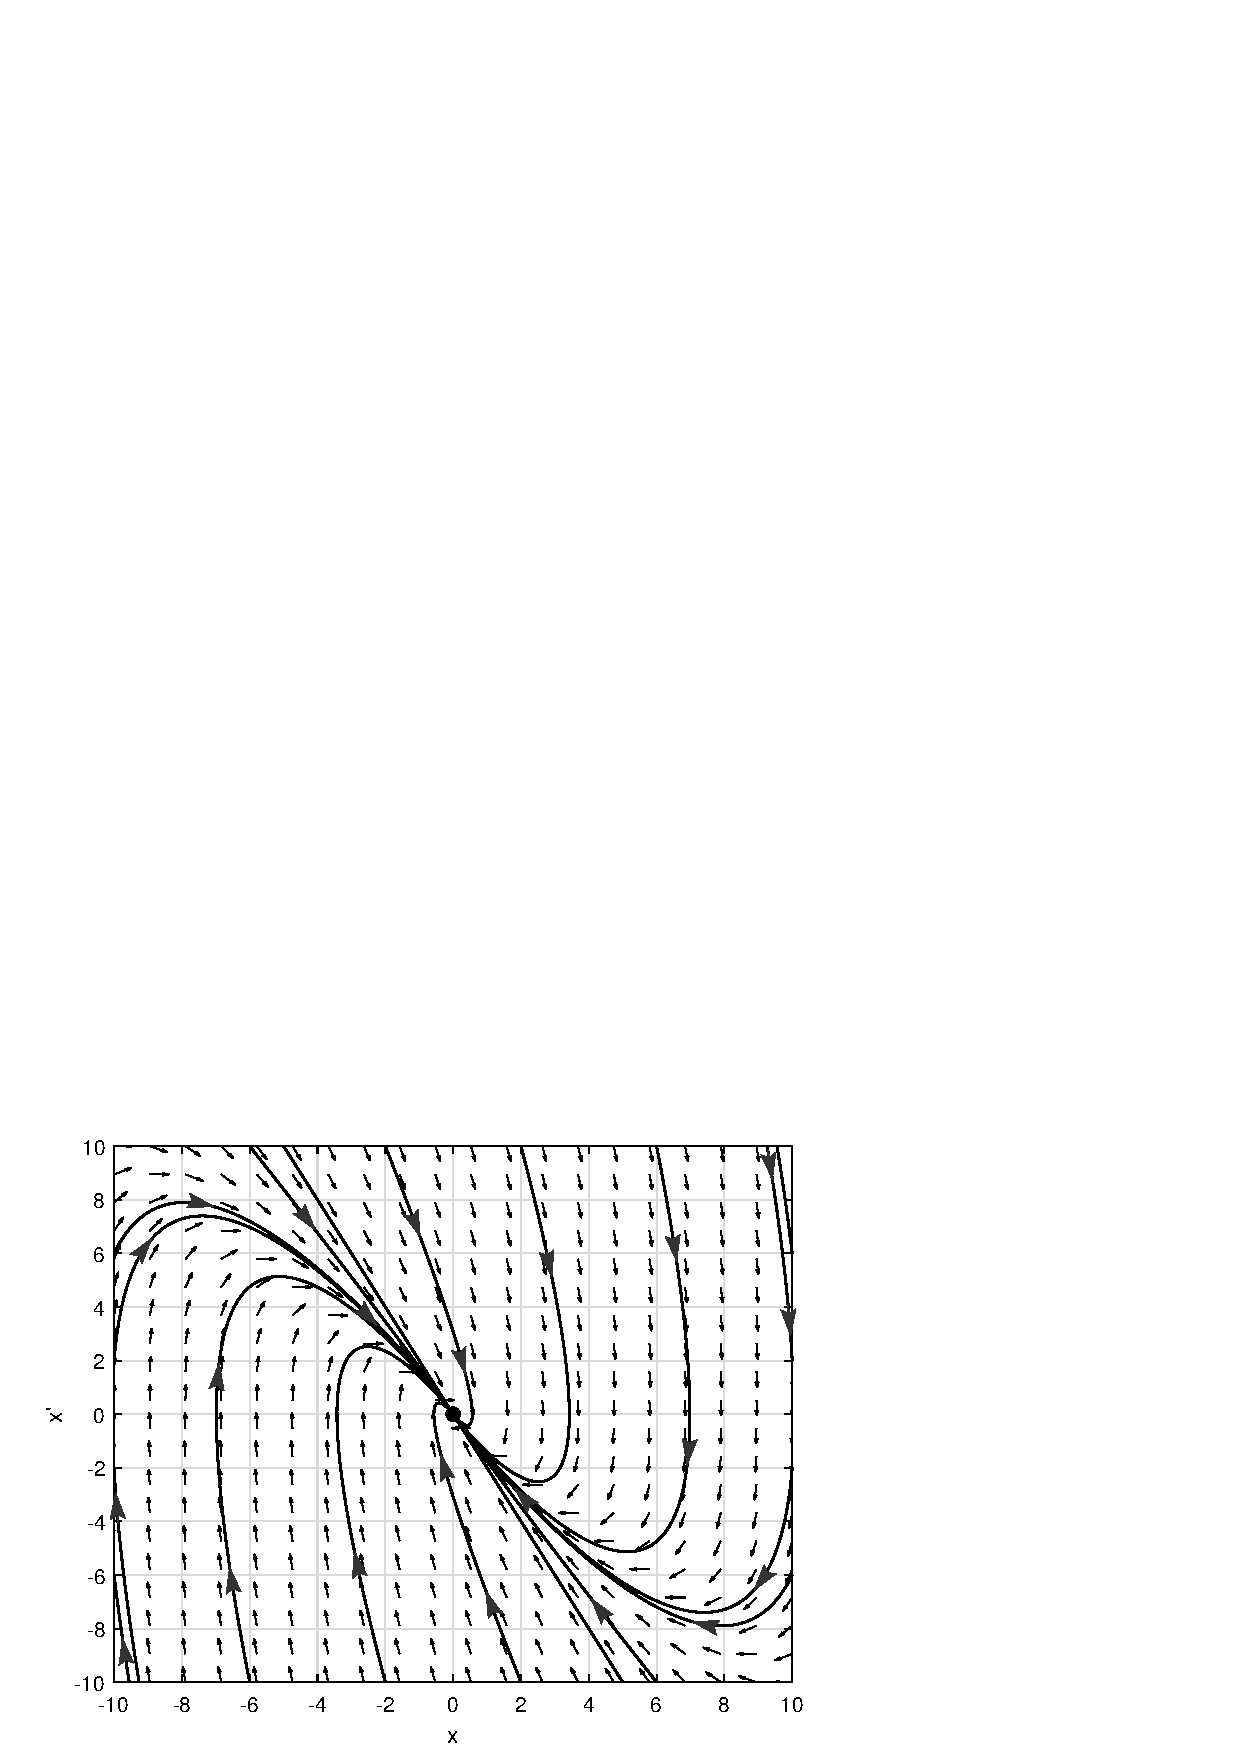
\includegraphics[width=0.5\linewidth]{fig/01_portrety_fazowe/wezel_stabilny.PNG}
            \caption{Ułożenie wartości własnych dla portretu typu \textbf{węzeł stabilny}.}
            \label{fig:enter-label}
        \end{figure}

        \begin{figure}[H]
            \centering
            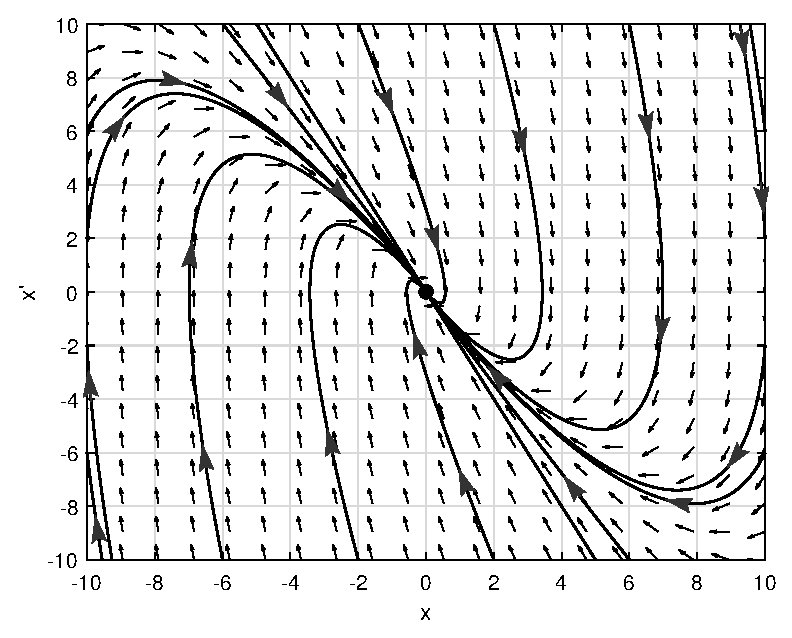
\includegraphics[width=0.75\linewidth]{fig/01_portrety_fazowe/wezel_stabilny.eps}
            \caption{Przykładowy portret fazowy dla portretu typu \textbf{węzeł stabilny}.}
            \label{fig:enter-label}
        \end{figure}

        \begin{figure}[H]
            \centering
            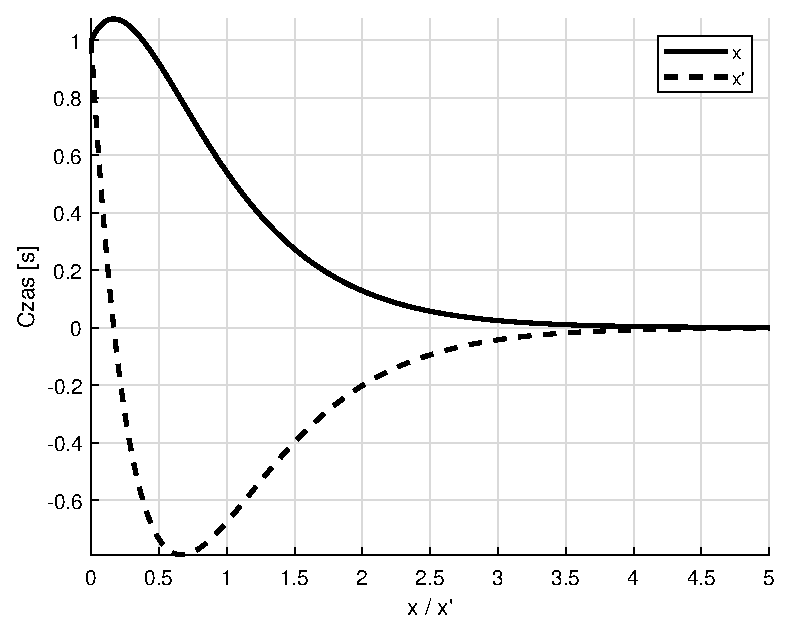
\includegraphics[width=0.5\linewidth]{fig/01_portrety_fazowe/wezel_stabilny_wykres.eps}
            \caption{Przykładowe przebiegi czasowe dla portretu typu \textbf{węzeł stabilny}.}
            \label{fig:enter-label}
        \end{figure}

        %------------------------------------------------------
        \subsubsection{Węzeł niestabilny - 2 pierwiastki rzeczywiste, dodatnie}
        Aby istniały dwa pierwiastki rzeczywiste, dodatnie muszą zachodzić warunki:
        \begin{itemize}
            \item $\xi < -1$ - tłumienie,
            \item $\omega_{0}^{2} < 0$.
        \end{itemize}

        \begin{figure}[H]
            \centering
            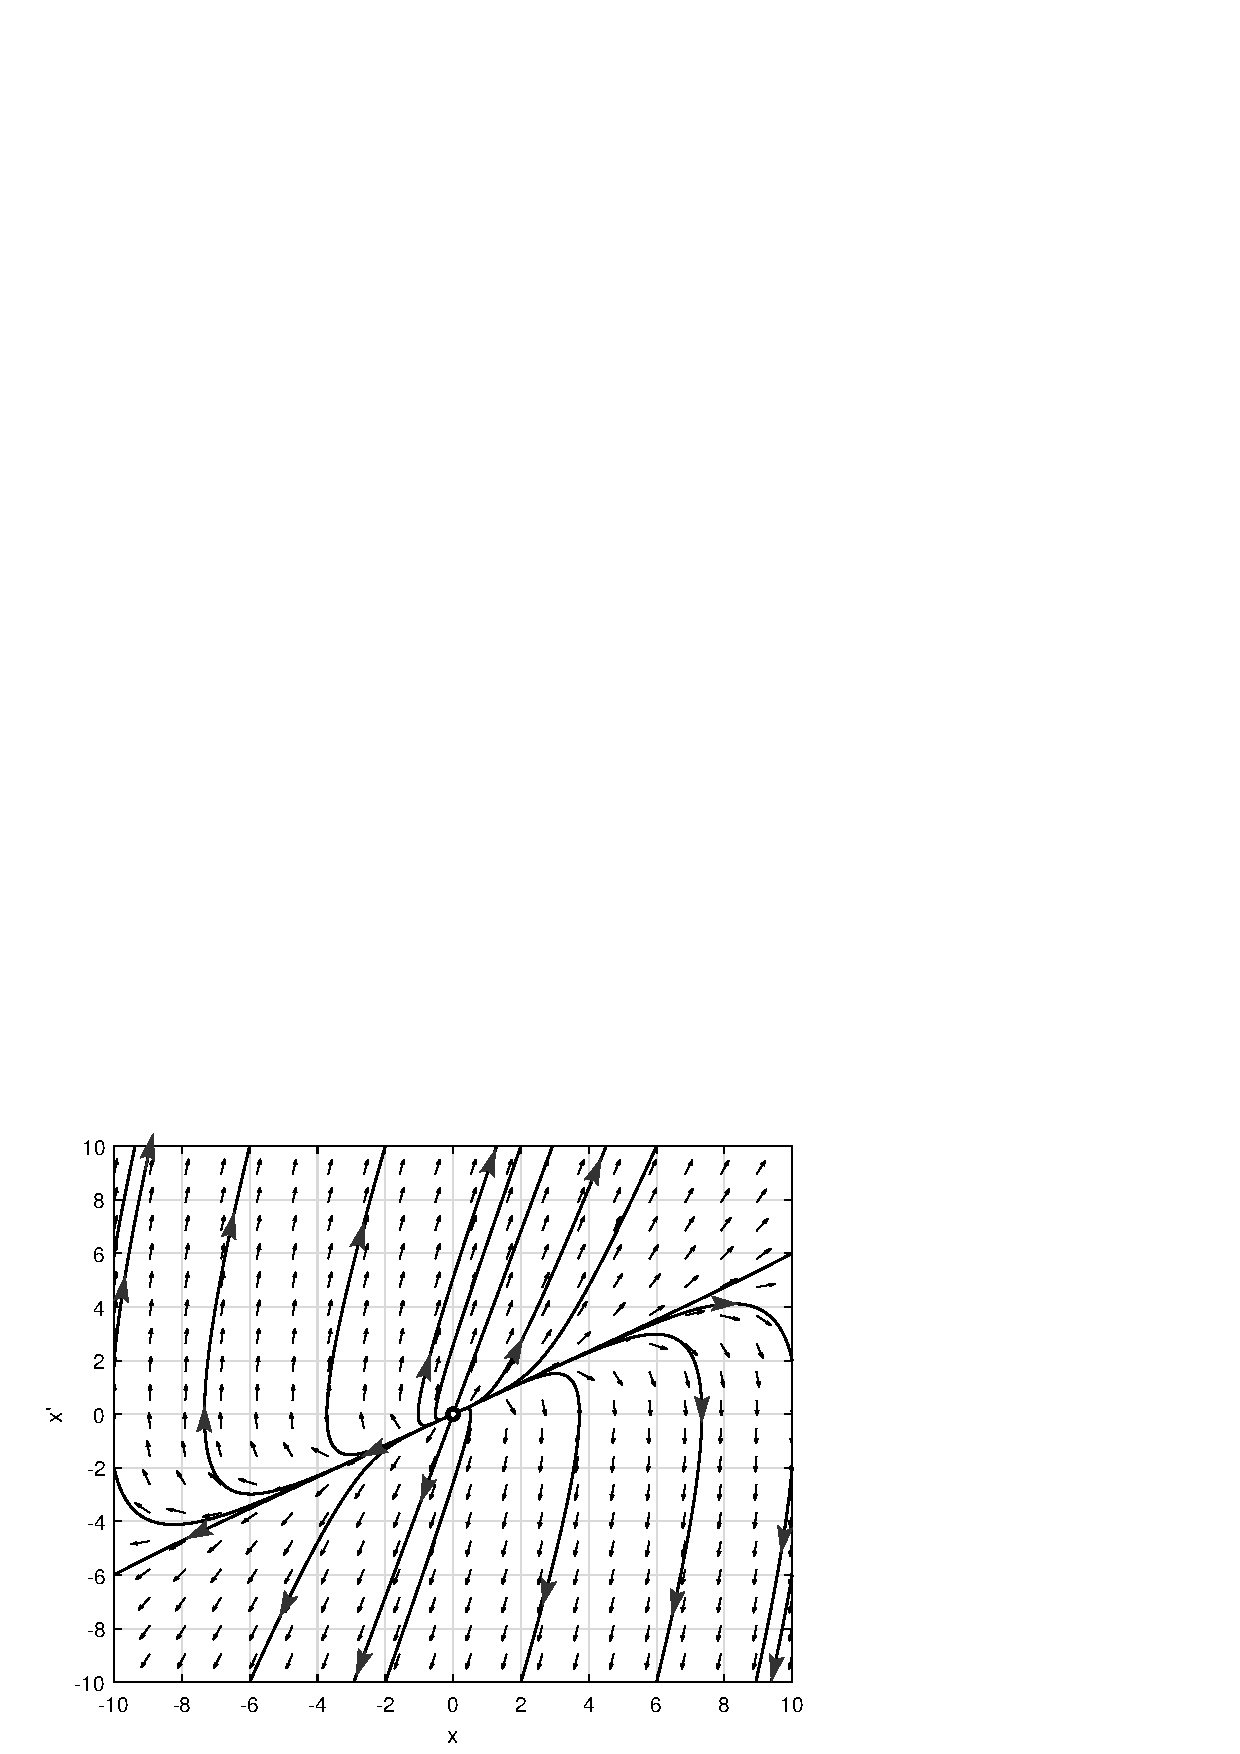
\includegraphics[width=0.5\linewidth]{fig/01_portrety_fazowe/wezel_niestabilny.PNG}
            \caption{Ułożenie wartości własnych dla portretu typu \textbf{węzeł niestabilny}.}
            \label{fig:enter-label}
        \end{figure}

        \begin{figure}[H]
            \centering
            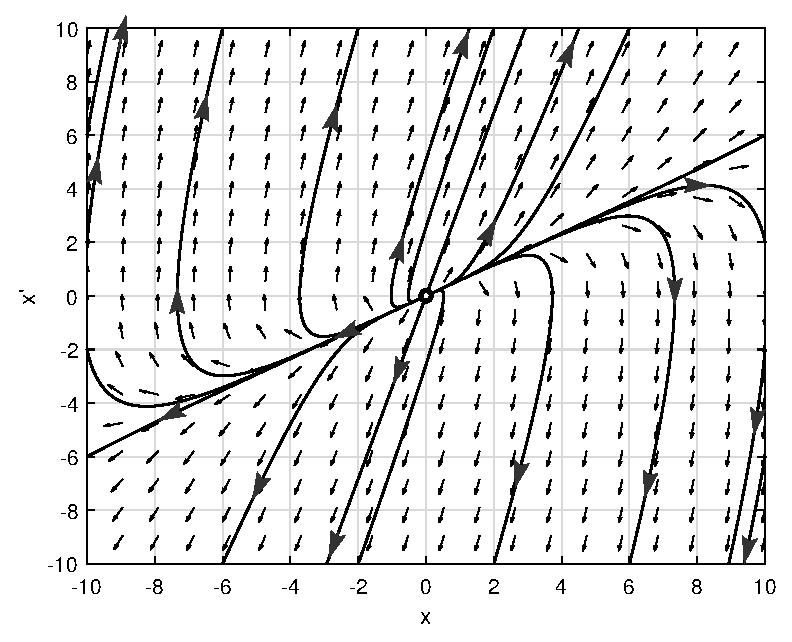
\includegraphics[width=0.75\linewidth]{fig/01_portrety_fazowe/wezel_niestabilny.eps}
            \caption{Przykładowy portret fazowy dla portretu typu \textbf{węzeł niestabilny}.}
            \label{fig:enter-label}
        \end{figure}

        \begin{figure}[H]
            \centering
            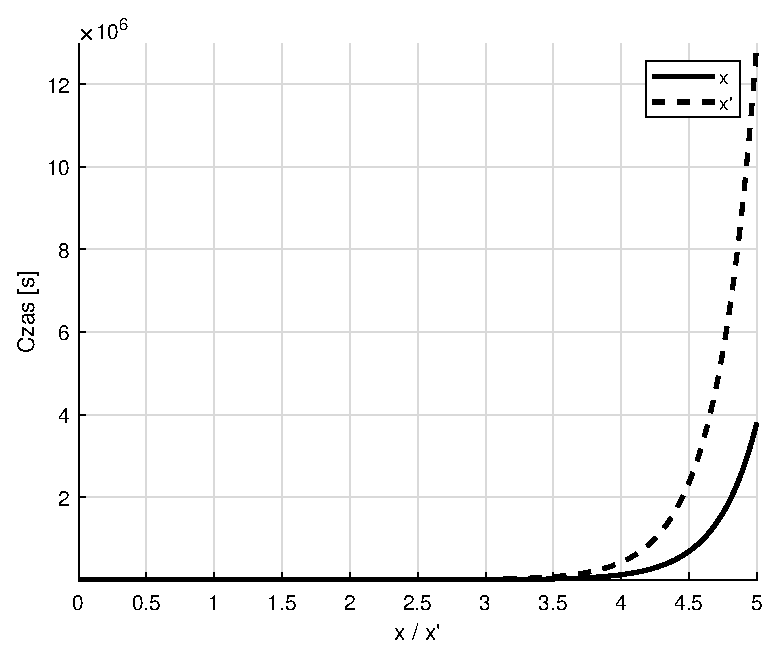
\includegraphics[width=0.5\linewidth]{fig/01_portrety_fazowe/wezel_niestabilny_wykres.eps}
            \caption{Przykładowe przebiegi czasowe dla portretu typu \textbf{węzeł niestabilny}.}
            \label{fig:enter-label}
        \end{figure}

        %------------------------------------------------------
        \subsubsection{Siodło - 2 pierwiastki rzeczywiste, przeciwnych znaków}
        Aby istniały dwa pierwiastki rzeczywiste, dodatnie muszą zachodzić warunki:
        \begin{itemize}
            \item $\xi = 0$ - tłumienie,
            \item $\omega_{0}^{2} < 0$.
        \end{itemize}

        \begin{figure}[H]
            \centering
            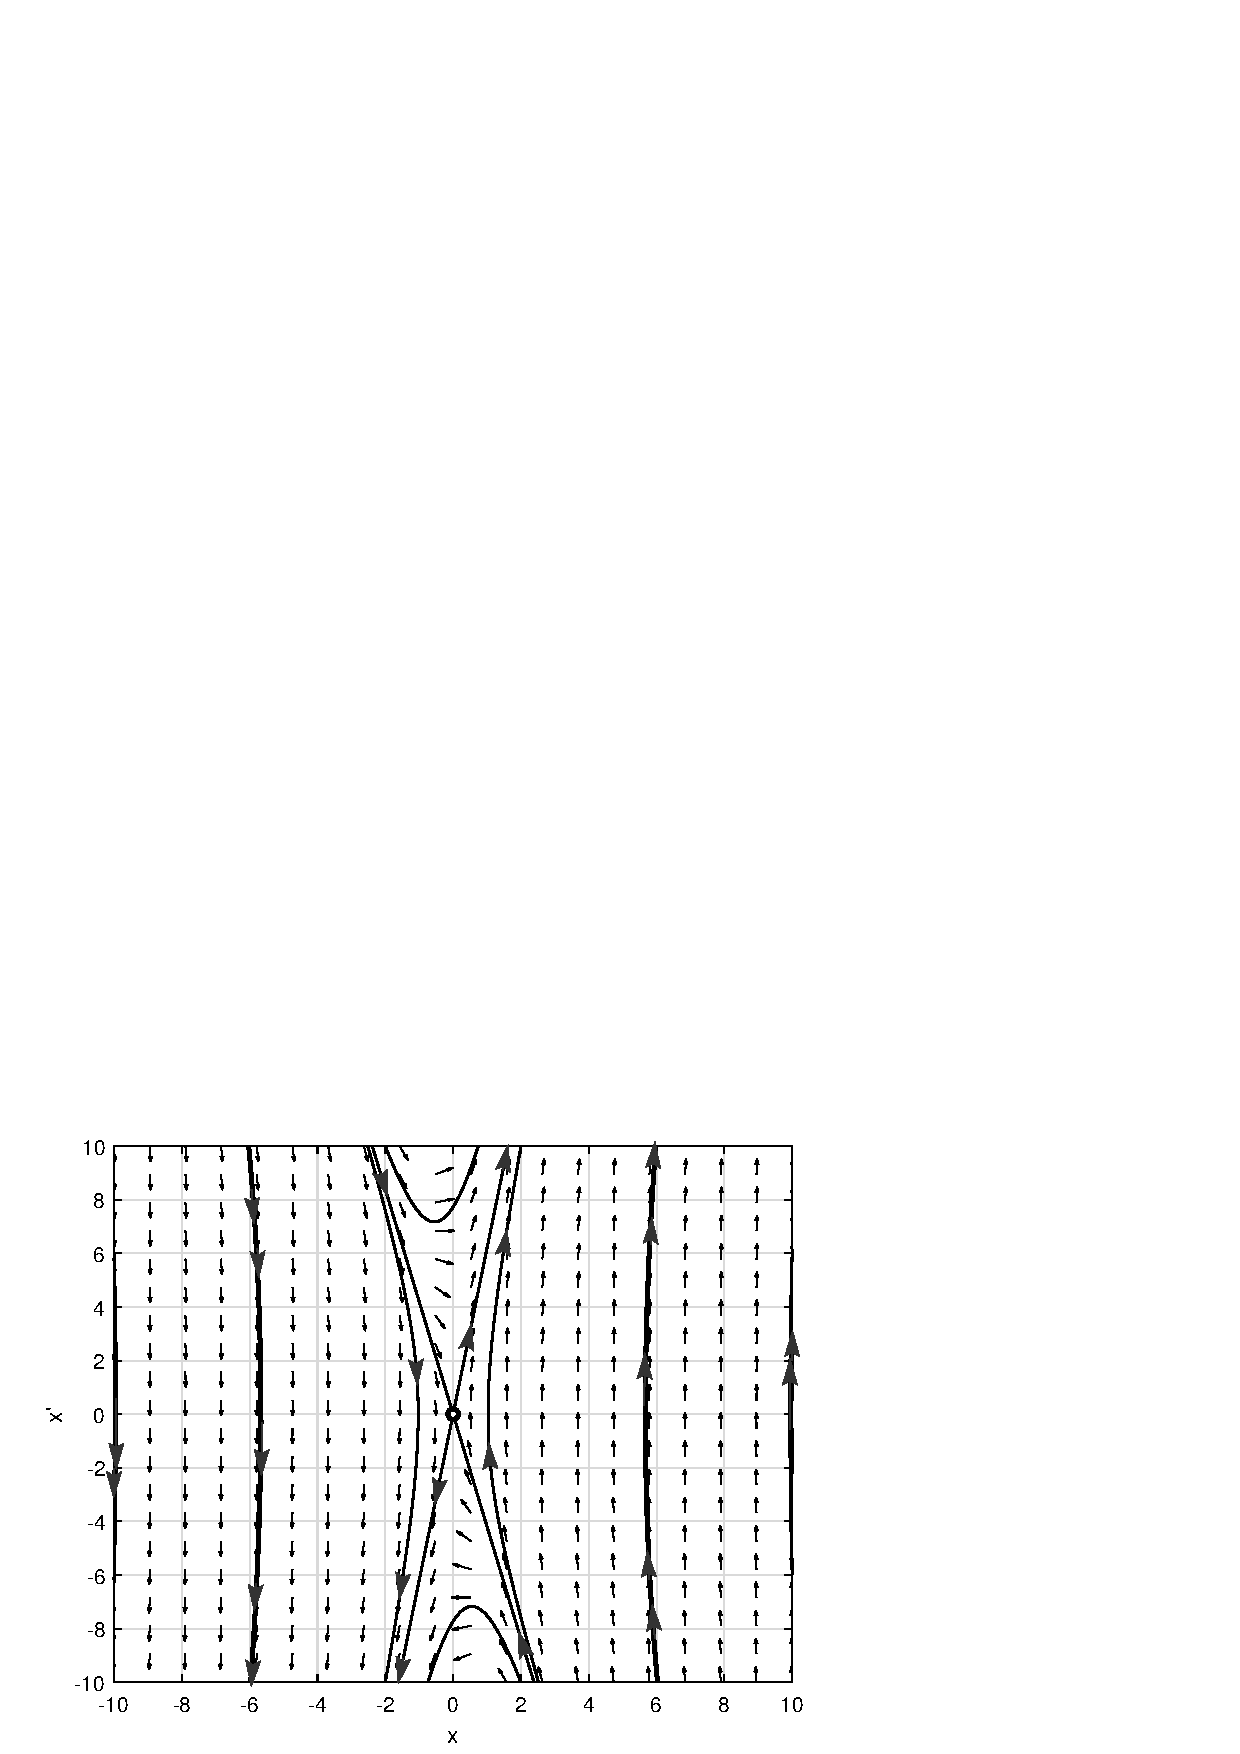
\includegraphics[width=0.5\linewidth]{fig/01_portrety_fazowe/siodlo.PNG}
            \caption{Ułożenie wartości własnych dla portretu typu \textbf{siodło}.}
            \label{fig:enter-label}
        \end{figure}

        \begin{figure}[H]
            \centering
            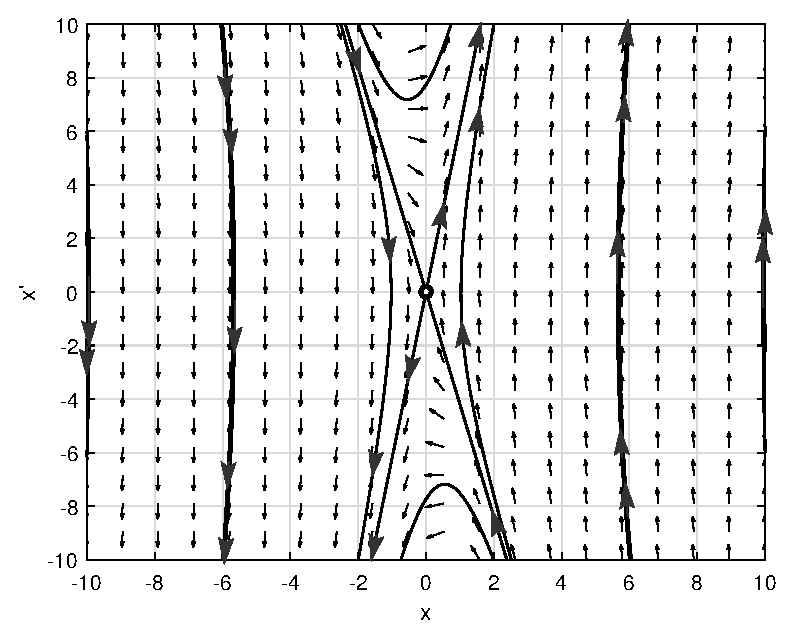
\includegraphics[width=0.75\linewidth]{fig/01_portrety_fazowe/siodlo.eps}
            \caption{Przykładowy portret fazowy dla portretu typu \textbf{siodło}.}
            \label{fig:enter-label}
        \end{figure}

        \begin{figure}[H]
            \centering
            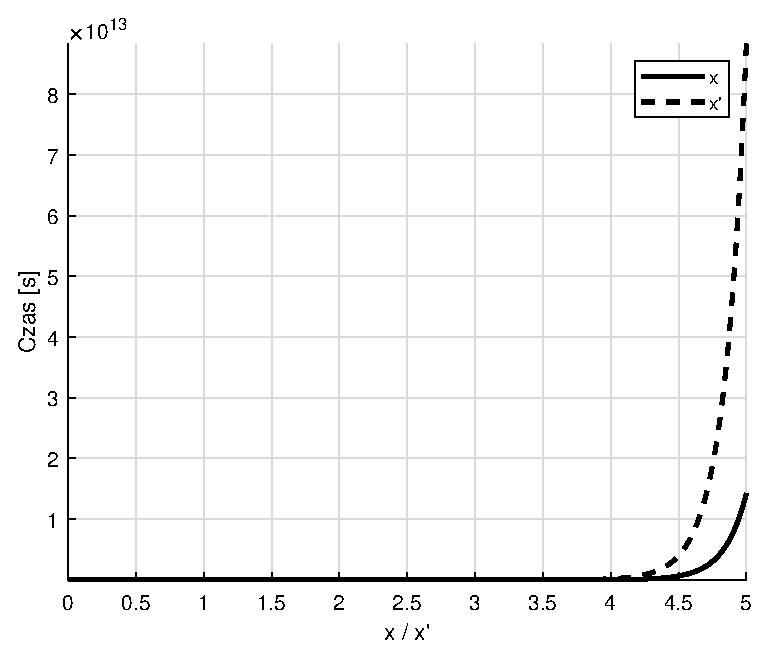
\includegraphics[width=0.5\linewidth]{fig/01_portrety_fazowe/siodlo_wykres.eps}
            \caption{Przykładowe przebiegi czasowe dla portretu typu \textbf{siodło}.}
            \label{fig:enter-label}
        \end{figure}

        %------------------------------------------------------
        \subsubsection{Jeden pierwiastek zerowy, jeden niezerowy}
        Aby istniały dwa pierwiastki rzeczywiste, dodatnie muszą zachodzić warunki:
        \begin{itemize}
            \item $\xi \neq 0$ - tłumienie,
            \item $\omega_{0} = 0$.
        \end{itemize}

        \begin{figure}[H]
            \centering
            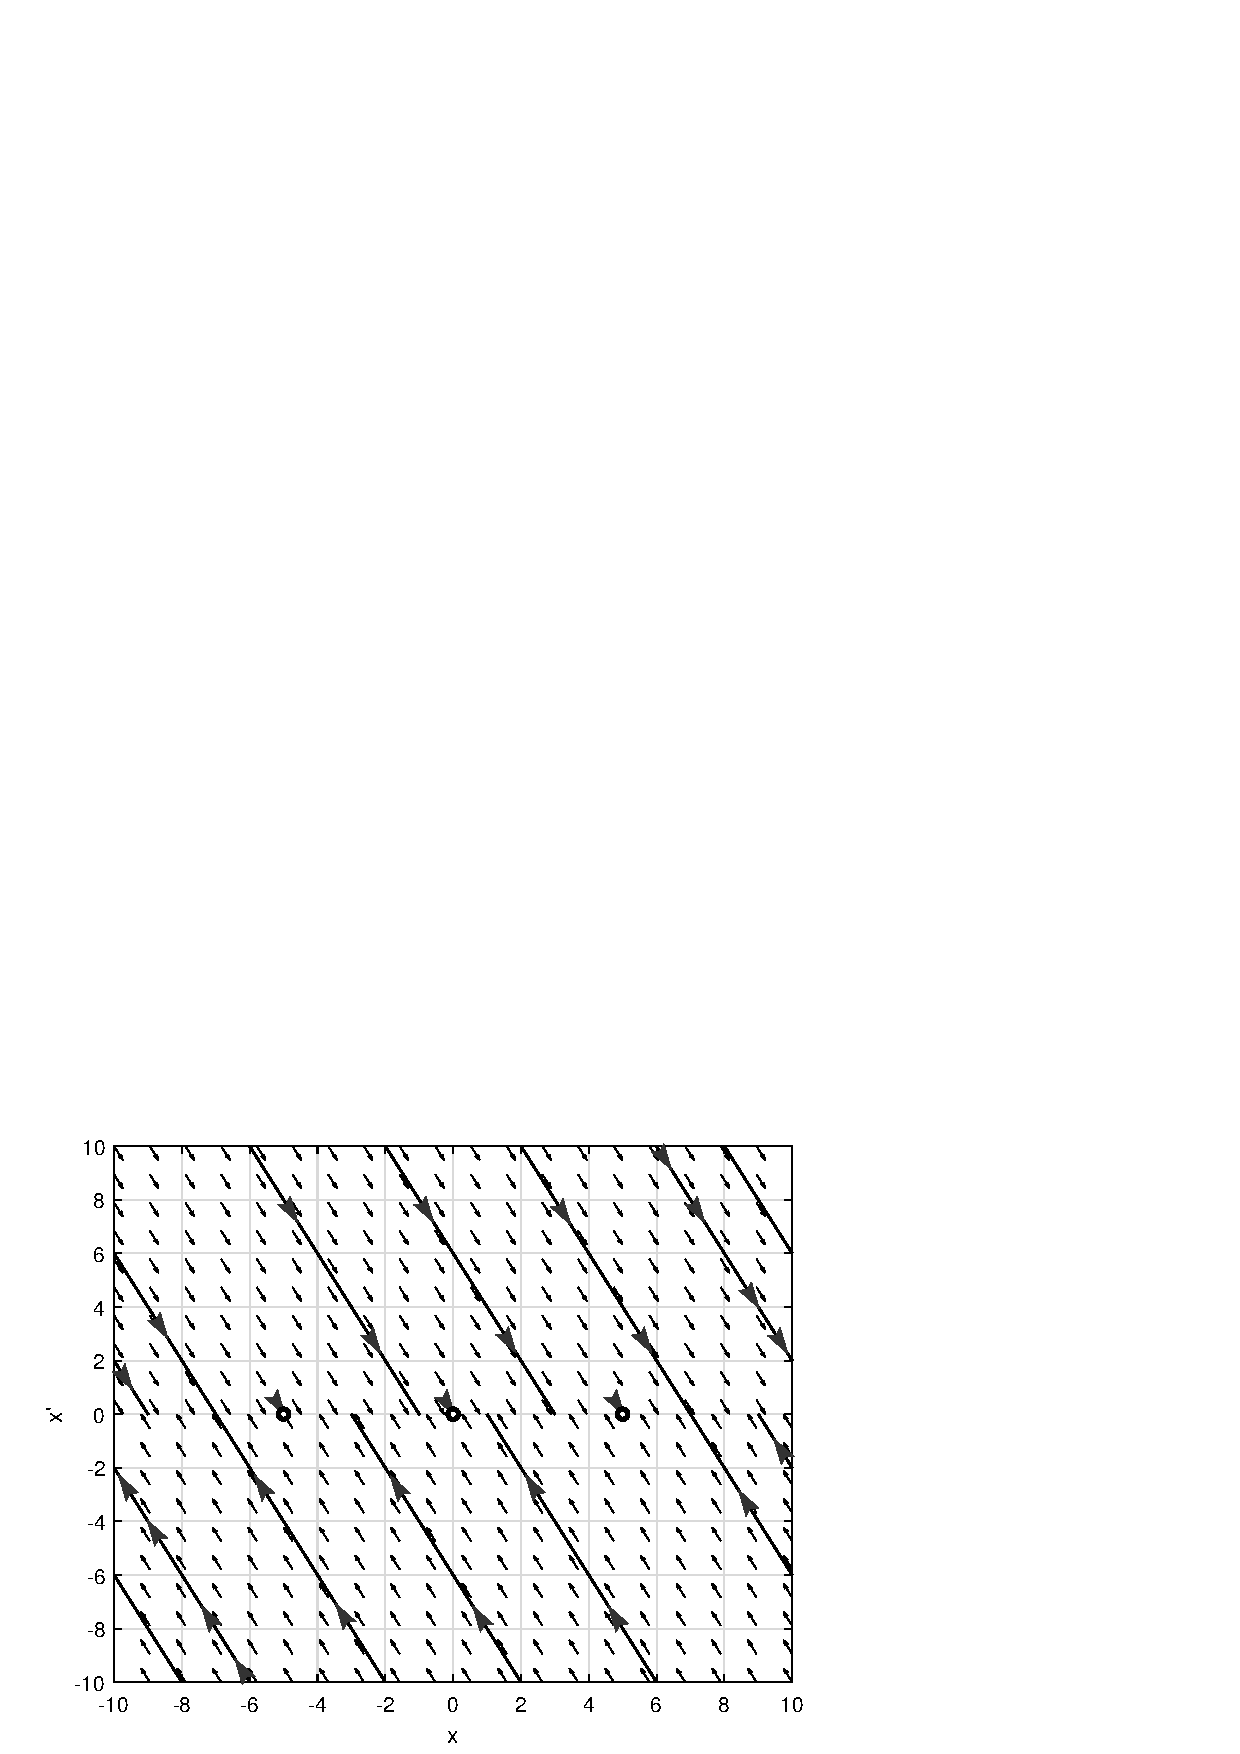
\includegraphics[width=0.3\linewidth]{fig/01_portrety_fazowe/jedno_zero.PNG}
            \caption{Ułożenie wartości własnych dla portretu dla układu \textbf{z jednym zerem}.}
            \label{fig:enter-label}
        \end{figure}

        \begin{figure}[H]
            \centering
            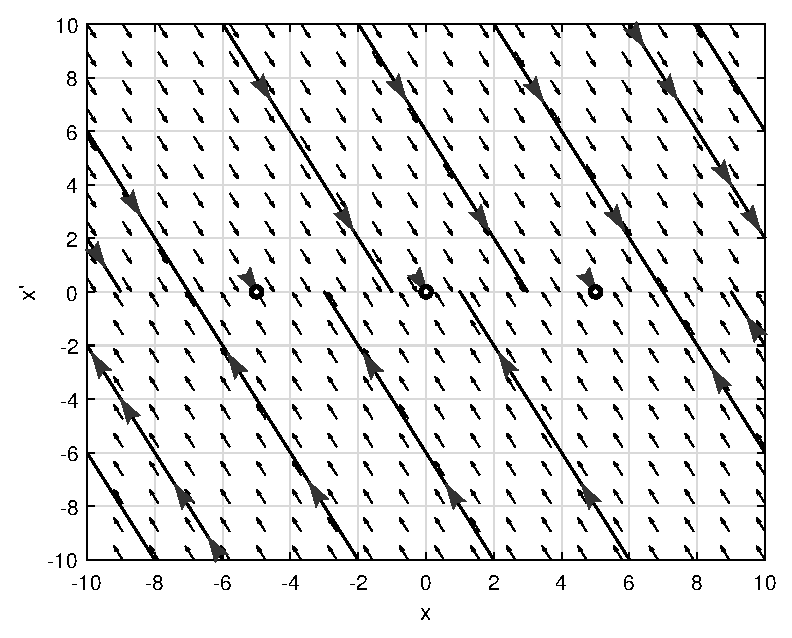
\includegraphics[width=0.75\linewidth]{fig/01_portrety_fazowe/jedno_zero.eps}
            \caption{Przykładowy portret fazowy dla \textbf{jednego pierwiastka równego 0}.}
            \label{fig:enter-label}
        \end{figure}

        \begin{figure}[H]
            \centering
            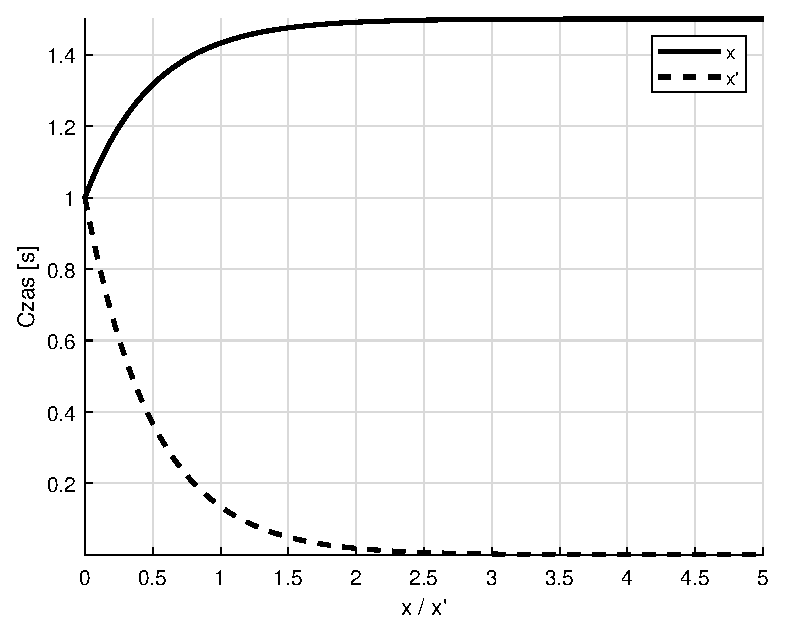
\includegraphics[width=0.5\linewidth]{fig/01_portrety_fazowe/jedno_zero_wykres.eps}
            \caption{Przykładowe przebiegi czasowe dla \textbf{jednego pierwiastka równego 0}.}
            \label{fig:enter-label}
        \end{figure}

        %------------------------------------------------------
        \subsubsection{Dwa pierwiastki zerowe - z jednym wektorem własnym}
        Aby istniały dwa pierwiastki rzeczywiste, dodatnie muszą zachodzić warunki:
        \begin{itemize}
            \item $\xi = 0$ - tłumienie,
            \item $\omega_{0} = 0$.
        \end{itemize}

        \begin{figure}[H]
            \centering
            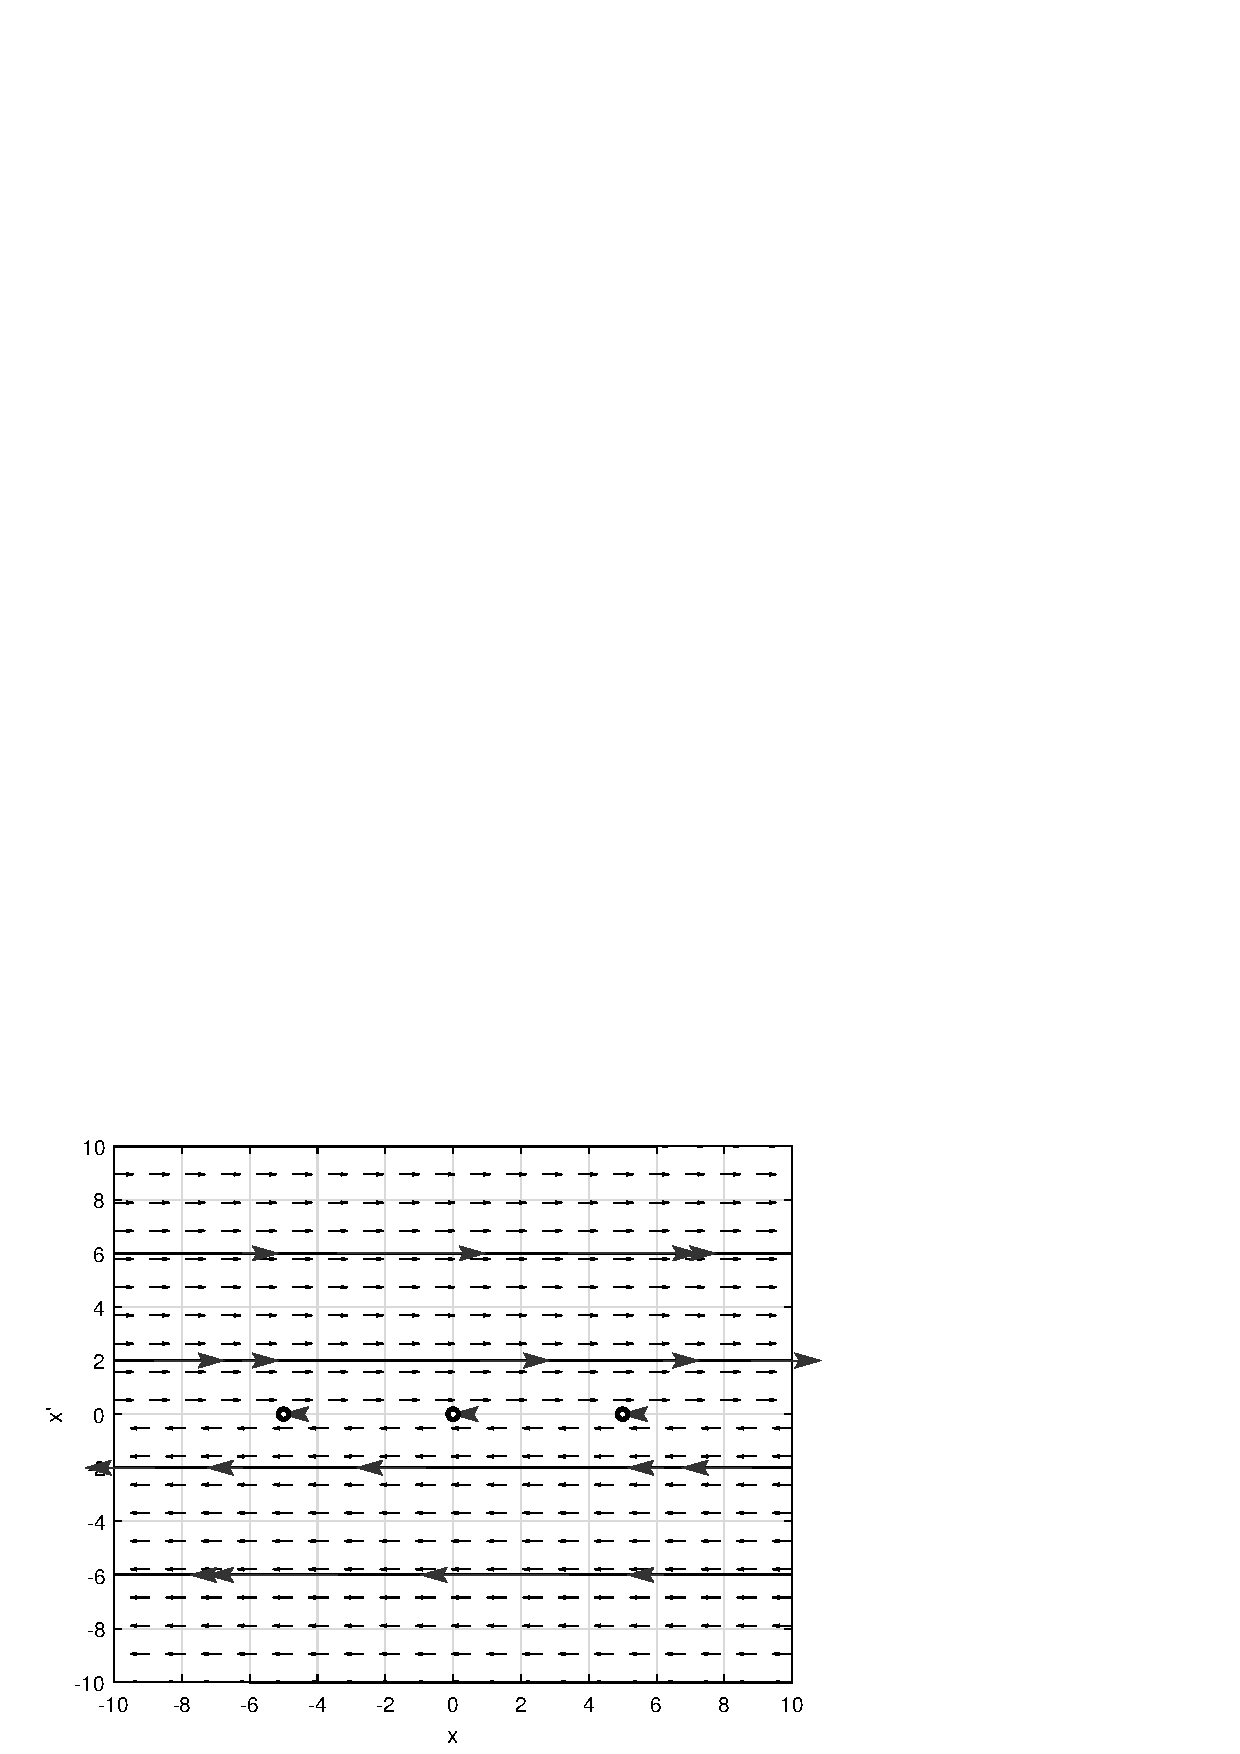
\includegraphics[width=0.3\linewidth]{fig/01_portrety_fazowe/dwa_zera.PNG}
            \caption{Ułożenie wartości własnych dla portretu dla układu \textbf{z dwoma zerami i jednym wektorem własnym}.}
            \label{fig:enter-label}
        \end{figure}

        \begin{figure}[H]
            \centering
            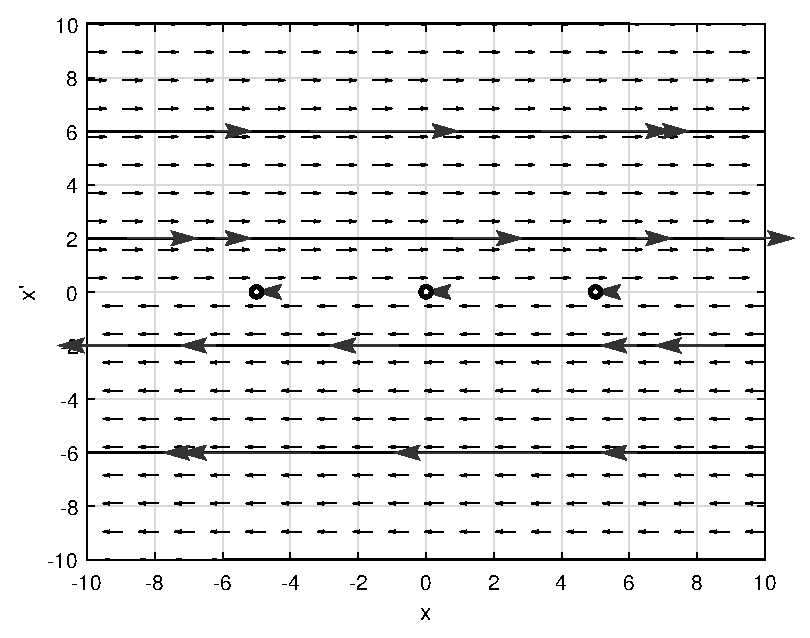
\includegraphics[width=0.75\linewidth]{fig/01_portrety_fazowe/dwa_zera.eps}
            \caption{Przykładowy portret fazowy dla \textbf{jednego pierwiastka równego 0}.}
            \label{fig:enter-label}
        \end{figure}

        \begin{figure}[H]
            \centering
            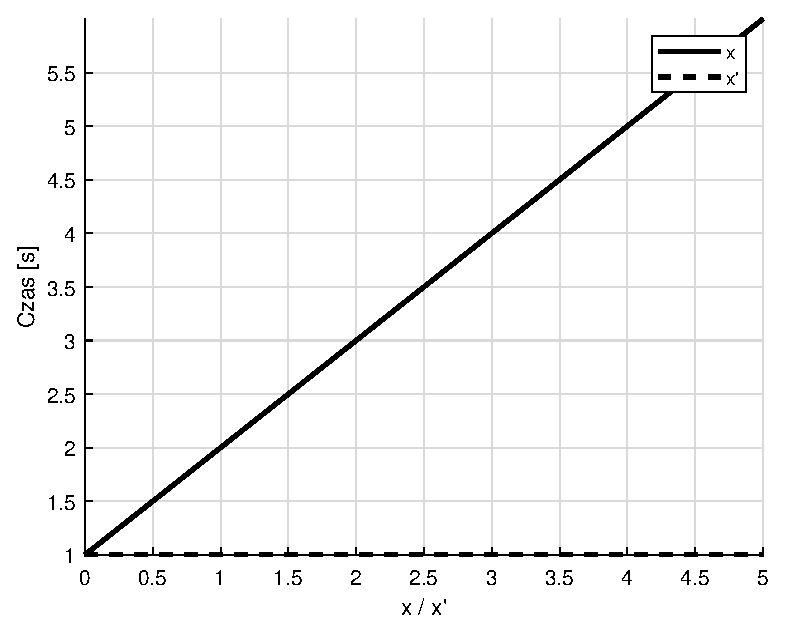
\includegraphics[width=0.5\linewidth]{fig/01_portrety_fazowe/dwa_zera_wykres.eps}
            \caption{Przykładowe przebiegi czasowe dla \textbf{dwóch pierwiastków równych 0 (z dwoma wektorami własnymi)}.}
            \label{fig:enter-label}
        \end{figure}

         %------------------------------------------------------
        \subsubsection{Dwa pierwiastki zerowe - z dwoma wektorami własnymi}
        Aby istniały dwa pierwiastki rzeczywiste, dodatnie muszą zachodzić warunki:
        \begin{itemize}
            \item $\xi = 0$ - tłumienie,
            \item $\omega_{0} = 0$.
        \end{itemize}
        Ten przypadek zachodzi tylko gdy $A = 0$.

        \begin{figure}[H]
            \centering
            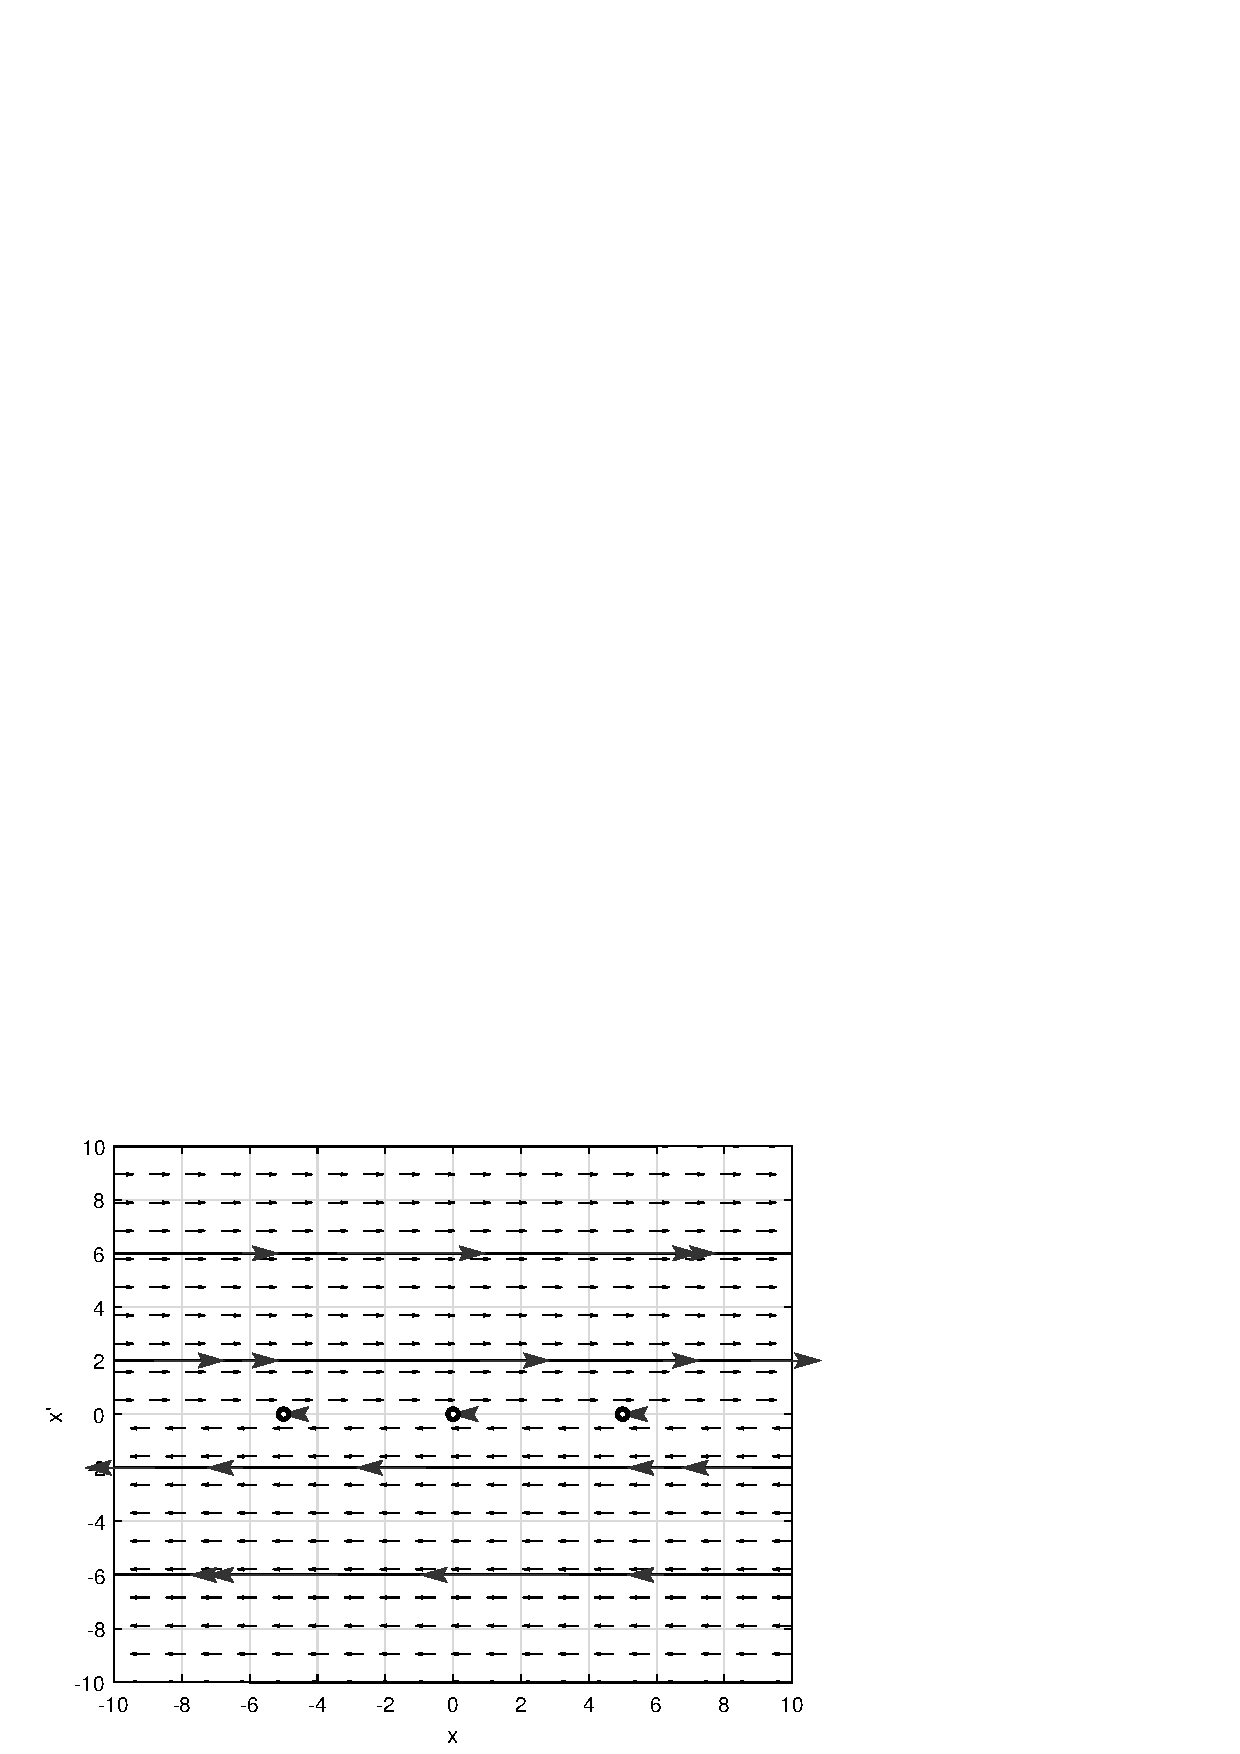
\includegraphics[width=0.3\linewidth]{fig/01_portrety_fazowe/dwa_zera.PNG}
            \caption{Ułożenie wartości własnych dla portretu dla układu \textbf{z dwoma zerami i dwoma wektorami własnymi}.}
            \label{fig:enter-label}
        \end{figure}

        \begin{figure}[H]
            \centering
            \includegraphics[width=0.75\linewidth]{fig/01_portrety_fazowe/dwa_zera_total.eps}
            \caption{Przykładowy portret fazowy dla \textbf{jednego pierwiastka równego 0}.}
            \label{fig:enter-label}
        \end{figure}

        \begin{figure}[H]
            \centering
            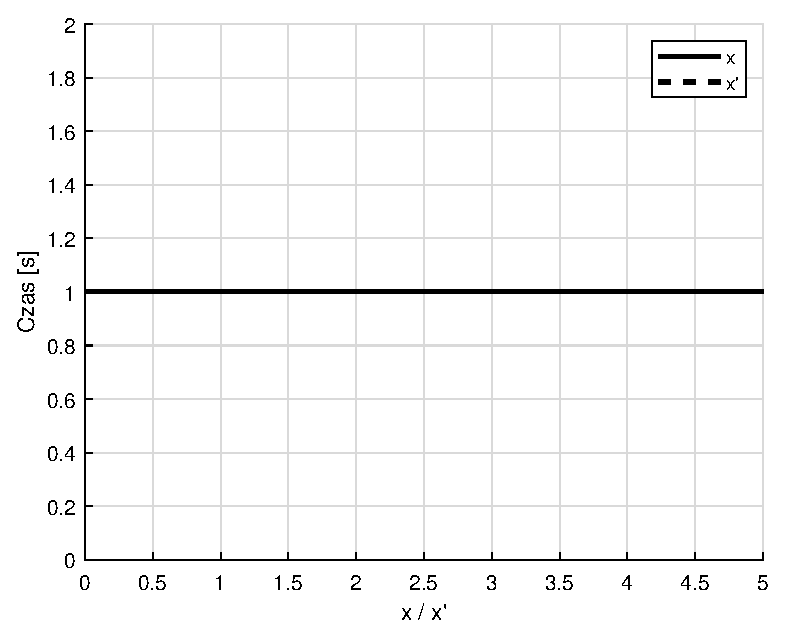
\includegraphics[width=0.5\linewidth]{fig/01_portrety_fazowe/dwa_zera_total_wykres.eps}
            \caption{Przykładowe przebiegi czasowe dla \textbf{dwóch pierwiastków równych 0 (z jednym wektorem własnym)}.}
            \label{fig:enter-label}
        \end{figure}
    
\section{Przebieg ćwiczenia}
\begin{enumerate}
    \item Przygotować 9 macierzy stanu - po jednej na każdy typ portretu fazowego. Dla każdej z macierzy podać ich wartości własne, postać Jordana, postać Frobeniusa.
    \item Skonstruować model Simulinka wykorzystujący blok \textit{State-Space}, do symulowania odpowiedzi układu.
    \begin{figure}[H]
        \centering
        \includegraphics[width=0.5\linewidth]{fig/01_portrety_fazowe/model_sinulink.PNG}
        \caption{Model symulacyjny.}
        \label{fig:enter-label}
    \end{figure}
    \item Wybrać zestaw warunków początkowych, i wyrysować odpowiedzi układu na płaszczyźnie fazowej dla każdego z nich - czyli portret fazowy. Wykonać to dla każdej z 9 macierzy przygotowanych w punkcie 1.
    W sprawozdaniu powinny się znaleźć:
    \begin{itemize}
        \item portrety fazowe dla macierzy, jej postaci Jordana i Frobeniusa - zaznaczyć wektory własne macierzy $A$ i skomentować ich znaczenie,
        \item zaznaczone zbiory punktów równowagi,
        \item przykłady przebiegów czasowych dla wybranych warunków początkowych,
        \item oszacowanie metodą aproksymacji łamaną czas stabilizacji - porównać czas z przebiegami czasowymi uzyskanymi symulacyjnie.
    \end{itemize}

    W sprawozdaniu zaznaczyć jak zmiana układu współrzędnych zmienia portret fazowy, jakie znaczenie mają wektory własne?
    
\end{enumerate}


%%%%%%%%%%%%%%%%%%%%%%%%%%%%%%%%%%%%%%%%%%%%%%%%%%%%%%%%%%%%
\newpage
\begin{thebibliography}{9}

\bibitem{Mitkowski2007}
  Mitkowski, W., Baranowski, J., Hajduk, K., Korytowski, A., Tutaj, A.,
  \emph{Teoria Sterowania: Materiały Pomocnicze do Ćwiczeń Laboratoryjnych},
  AGH Uczelniane wydawnictwo Naukowo-Dydaktyczne,
  2007.

\bibitem{Amborski1978}
  Amborski, K., Marusak, A.,
  \emph{Teoria Sterowania w Ćwiczeniach},
  Państwowe Wydawnictwo Naukowe,
  1978.

\bibitem{Gessing1981}
  Gessing, R., Latarnik, M., Skrzywan-Kossek, A.,
  \emph{Zbiór Zadań z Teorii Nieliniowych Układów Regulacji i Sterowania},
  Wydawnictwo Naukowo-Techniczne,
  1981.

\bibitem{Gibson1968}
  Gibson, J. E.,
  \emph{Nieliniowe Układy Sterowania Automatycznego},
  Wydawnictwo Naukowo-Techniczne,
  1968.

\end{thebibliography}

\end{document}
